% ******************* PhD Thesis Presentation Template *************************
% Please have a look at the README.md file for info on how to use the template
\PassOptionsToPackage{table}{xcolor} % <-μονο εδω δουλεύει!!

\documentclass[aspectratio=169,progrbar,draft]{Classes/beamerLct}%%  
% ******************************************************************************
% ******************************* Class Options ********************************
% *********************** See README for more details **************************
% ******************************************************************************
%
% `aspectratio=169`: reduce ratio to 16:9
%
% `customfont`: Pre-defined font is "Biolinum O". This option enable custom fonts .
% Config custom fonts at `preamble.tex`. Custom font include GFS package.
%
% `10pt` or `11pt`(default) : Recommended font size. Smaller (`8pt`,`9pt`)
% or huge (`14pt`,`17pt`,`20pt`) font size are NOT recommended except special cases.
%
% `draft`: Special draft mode with line numbers, images, and water mark with 
% timestamp and custom text. Position of the text can also be modified. To 
% disable figures see on `preample.tex` the Draftmode section.
%
% `chapter`: This option enables only the specified chapter and it's references
% Useful for review and corrections.
%
% `notes`: Prints frames and notes 
%
% `notes=only`: Prints only notes of each frame
%
% `printbib`: Include bibliography at the end of the presentation 
%
% `progrbar`: Enable progress bar in the frame. Chose this option after your 
% first compilation. Disable on chapter mode.

% ********************************** Preamble **********************************
% Preamble: Contains packages and user-defined commands and settings
% ********************************** Preamble **********************************
% Preamble: Contains packages and user-defined commands and settings

%%-----------------------------------------------------------------------------
%% USE THEME
%%-----------------------------------------------------------------------------
\usetheme{RedLecture}
% \usetheme{PaloAlto} 
% \usetheme{Singapore}
% \usetheme{Szeged}
% \usetheme{CambridgeUS}
% \usetheme{Montpellier}
% \usetheme{Pittsburgh} <---
% \usetheme{Warsaw}
% \usetheme{Rochester}
% \usetheme{Marburg}
% \usetheme{Malmoe}
% \usetheme{Madrid}
% \usetheme{Luebeck}
% \usetheme{Ilmenau}
% \usetheme{Hannover} <---
% \usetheme{Goettingen}
% \usetheme{Dresden}
% \usetheme{boxes}
% \usetheme{Boadilla}
% \usetheme{Berlin}
% \usetheme{Berkeley}
% \usetheme{AnnArbor}

\usepackage{lmodern}
\usepackage[scale=2]{ccicons}

%%-----------------------------------------------------------------------------
%%  double slides left presentation // right notes NOT WORK WELL!!!
%%-----------------------------------------------------------------------------
% \usepackage{pgfpages}
% \setbeameroption{show notes on second screen=right}

%%-----------------------------------------------------------------------------
% %  margins
%%-----------------------------------------------------------------------------
\setbeamersize{text margin left=0.4cm}  % <- like this
\setbeamersize{text margin right=0.4cm} % <- like this

%%-----------------------------------------------------------------------------
%% Set background for simpledso theme
%%-----------------------------------------------------------------------------
%\graphicspath{{Chapter3/Figs/Vector/}{Chapter3/Figs/}}
\setwatermark{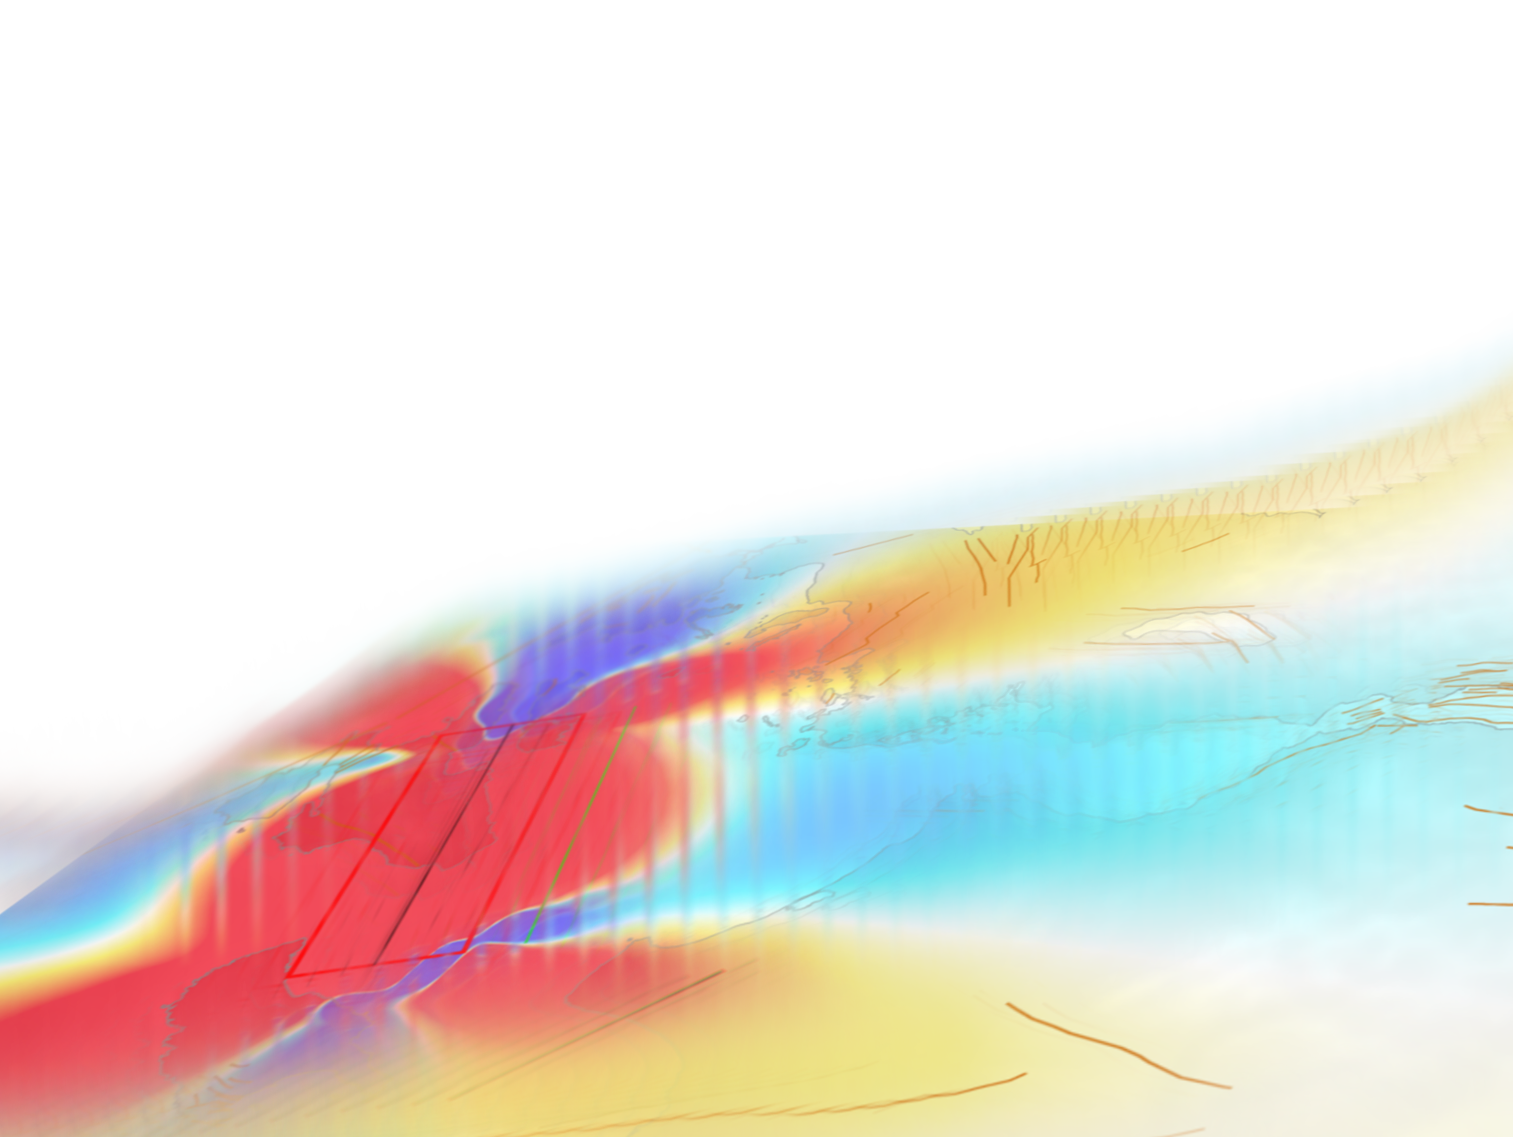
\includegraphics[height=12cm,draft=false]{Figs/kef_1953_kef.png}}

%%-----------------------------------------------------------------------------
%% Languages
%%-----------------------------------------------------------------------------
% \usepackage[english, greek]{babel}
\usepackage{xgreek}
\usepackage[Greek,Latin]{ucharclasses}
\setTransitionsForGreek{\setlanguage{greek}}{\setlanguage{english}}
% \usepackage{xunicode}
% \usepackage{xltxtra}
% \usepackage[monogreek]{xgreek}
% \usepackage{tabu}

%%-----------------------------------------------------------------------------
%% Tables
%%-----------------------------------------------------------------------------
\usepackage{booktabs,tabularx}
\usepackage{tabu}
\usepackage{multirow}

%%-----------------------------------------------------------------------------
%% Fonts
%%-----------------------------------------------------------------------------

% Add `customfont' in the document class option to use this section
\ifdefineCustomFont
  \usepackage{fontspec}
  \usefonttheme{professionalfonts} % using non standard fonts for beamer
  \usefonttheme{serif} % default family is serif
%  \setmainfont[Mapping=tex-text]{GFS Didot}
%  \setmainfont[Mapping=tex-text]{GFS Bodoni}
%  \setmainfont[Mapping=tex-text]{GFS Olga} % ότι να ναι αυτή!!πλάγια NOT support English
  \setmainfont[Mapping=tex-text]{GFS Neohellenic}
%  \setmainfont[Mapping=tex-text]{GFS Artemisia}
%  \setmainfont[Mapping=tex-text]{GFS Elpis} %low resolution printing


%%  % For use with XeLaTeX, enable Libertine
%    \setmainfont[
%      Path              = /usr/share/texlive/texmf-dist/fonts/opentype/public/libertine/, %./libertine/opentype/,
%      Extension         = .otf,
%      UprightFont = LinLibertine_R,
%      BoldFont = LinLibertine_RZ, % Linux Libertine O Regular Semibold
%      ItalicFont = LinLibertine_RI,
%      BoldItalicFont = LinLibertine_RZI, % Linux Libertine O Regular Semibold Italic
%    ]
%    {LGR}
%  %  % load font from system font
%     \newfontfamily\libertinesystemfont{Linux Libertine O}

%  %% use xetex, enable Biolinum Fonts
%  \setmainfont[
%      Path              = /usr/share/texlive/texmf-dist/fonts/opentype/public/libertine/, %./libertine/opentype/,
%      Extension         = .otf,
%      UprightFont = LinBiolinum_R,
%      BoldFont = LinBiolinum_RB, % Linux Libertine O Regular Semibold
%      ItalicFont = LinBiolinum_RI,
%      %BoldItalicFont = LinBiolinum_RZI, % Linux Libertine O Regular Semibold Italic
%    ]
%    {LGR}
%  %  % load font from system font
%     \newfontfamily\libertinesystemfont{Linux Biolinum O}


\else
  \usepackage{fontspec}
  \usefonttheme{professionalfonts} % using non standard fonts for beamer
  \usefonttheme{serif} % default family is serif
%
%  %% Use Computer Modern Unicode Fonts, Support Greek Font
%  \setmainfont[Mapping=tex-text, Scale=0.90]{CMU Serif}
%  \setsansfont[Mapping=tex-text, Scale=0.90]{CMU Sans Serif}
%  \setmonofont{CMU Typewriter Text}
 
%%************* Latin Modern, not support greek*****************************
 \usepackage{lmodern}
 \usepackage[T1]{fontenc}
     
\fi % custom font class

%%-----------------------------------------------------------------------------
%% REQUIRED PACKAGES
%%-----------------------------------------------------------------------------
\usepackage{graphicx}  % Required for including images
\usepackage{fancybox}
% \usepackage{xcolor}
%% for tikz
% \usepackage{dtklogos}
%\usepackage{tikz}
\usetikzlibrary{mindmap,shadows}
\usepackage{smartdiagram}

% restart numbering footnotes per page
\usepackage{perpage}
\MakePerPage{footnote}
% % Sychronize footnotes on columns minipages
\renewcommand\thempfootnote{\arabic{mpfootnote}}

% use nice itemlists ..
%\usepackage{enumitem, color, amssymb}
\usepackage{url}
\hypersetup{colorlinks,citecolor=blue,linkcolor=,urlcolor=links}
%\hypersetup{colorlinks=true,allcolors=blue}

% use metalogo to print xelatex!
\usepackage{metalogo}

% % tcolorbox custom block, problem with caption package, cant solve it yet!
% \usepackage[most]{tcolorbox}

%%-----------------------------------------------------------------------------
%% Adgust figures
%%-----------------------------------------------------------------------------
\usepackage{adjustbox} % for \adjincludegraphics
% {\shadowbox{\color{black!35}\includegraphics[height=4cm]{img/iono.eps}}

%%-----------------------------------------------------------------------------
%% Print Arrows
%%-----------------------------------------------------------------------------
\usepackage{marvosym} % \MVRIGHTarrow
\usepackage{stmaryrd} % \shortrightarrow $\Rightarrow$
\usepackage{textcomp} % \textrightarrow

%%-----------------------------------------------------------------------------
%% Math symbols
%%-----------------------------------------------------------------------------
\usepackage{amssymb} 
\usepackage{amsmath}

% \usepackage{soul}
% \definecolor{lightblue}{rgb}{.90,.95,1}
% \sethlcolor{lightblue}
% \renewcommand<>{\hl}[1]{\only#2{\beameroriginal{\hl}}{#1}}
%% -----------------------------------------------------------------------------
%% CAPTIONS
%%-----------------------------------------------------------------------------
\usepackage{caption}
\usepackage{subcaption}
\captionsetup[figure]{font=footnotesize,labelfont=footnotesize,skip=0pt,belowskip=0pt}
\setbeamertemplate{caption}[numbered]

\setbeamerfont{caption}{size=\scriptsize}

%%-----------------------------------------------------------------------------
%% Four Quad
%%-----------------------------------------------------------------------------
\newcommand\FourQuad[4]{
    \begin{minipage}[b][.45\textheight][t]{.50\textwidth}\centering#1\end{minipage}\hfill%
    \begin{minipage}[b][.45\textheight][t]{.50\textwidth}\centering#2\end{minipage}\\[0.1cm]
    \begin{minipage}[b][.45\textheight][t]{.50\textwidth}\centering#3\end{minipage}\hfill
    \begin{minipage}[b][.45\textheight][t]{.50\textwidth}\centering#4\end{minipage}%
}

%%-----------------------------------------------------------------------------
%% Custom symbols for itemize
%%-----------------------------------------------------------------------------

\newenvironment{proenv}{\only{\setbeamercolor{local structure}{fg=green}}}{}
\newenvironment{conenv}{\only{\setbeamercolor{local structure}{fg=red}}}{}
 \usepackage{fontawesome}

%%-----------------------------------------------------------------------------
%% Rotate text
%%-----------------------------------------------------------------------------
\usepackage{rotating}
%\begin{turn}{45} 
% ...
% \end{turn}


%%-----------------------------------------------------------------------------
%% BIBLATEX
%%-----------------------------------------------------------------------------
\usepackage{hyperref}
\usepackage[backend=biber,
            style=authoryear,
            maxbibnames=9,
            maxcitenames=1,
            citestyle=authoryear,
            hyperref=true,
            backref=true,
            sorting=nty,
            natbib=true]{biblatex}

% Hypper linc for all citations use \parencite & \textcite
\ExecuteBibliographyOptions{maxcitenames=1}

\DeclareFieldFormat{citehyperref}{%
  \DeclareFieldAlias{bibhyperref}{noformat}% Avoid nested links
  \bibhyperref{#1}}

\DeclareFieldFormat{textcitehyperref}{%
  \DeclareFieldAlias{bibhyperref}{noformat}% Avoid nested links
  \bibhyperref{%
    #1%
    \ifbool{cbx:parens}
      {\bibcloseparen\global\boolfalse{cbx:parens}}
      {}}}

\savebibmacro{cite}
\savebibmacro{textcite}

\renewbibmacro*{cite}{%
  \printtext[citehyperref]{%
    \restorebibmacro{cite}%
    \usebibmacro{cite}}}

\renewbibmacro*{textcite}{%
  \ifboolexpr{
    ( not test {\iffieldundef{prenote}} and
      test {\ifnumequal{\value{citecount}}{1}} )
    or
    ( not test {\iffieldundef{postnote}} and
      test {\ifnumequal{\value{citecount}}{\value{citetotal}}} )
  }
    {\DeclareFieldAlias{textcitehyperref}{noformat}}
    {}%
  \printtext[textcitehyperref]{%
    \restorebibmacro{textcite}%
    \usebibmacro{textcite}}}



\bibliography{References/triangleref.bib}
\newcounter{bibitmctr}
\newcommand{\brf}{%
  \stepcounter{bibitmctr}%
  \ifnum\value{bibitmctr}=7%
    \setcounter{bibitmctr}{0}
    \framebreak
  \fi
}

\renewbibmacro*{finentry}{\finentry\brf}

% % cahnge fontsize of bibliography for biblatex
\renewcommand*{\bibfont}{\tiny}


%%-----------------------------------------------------------------------------
%% Insert frame after new section
%%-----------------------------------------------------------------------------
%% comment next lines if you don't like to use this
\AtBeginSection[]{
  \begin{frame}[b]
  \vspace{\fill}
  \centering
  \begin{beamercolorbox}[sep=8pt,center,shadow=true,rounded=true]{title}
     \usebeamerfont{title}\Large{\insertsectionhead}%
  \end{beamercolorbox}
  \vskip-2cm
  \begin{flushleft}
    {\color{blue!20}\rule{0.7\textwidth}{1pt}}\par
    {\color{blue!40}\rule{0.5\textwidth}{1pt}}\par
    {\color{blue!60}\rule{0.3\textwidth}{1pt}}\par
    {\color{blue!70}\rule{0.16\textwidth}{1pt}}\par
    {\color{blue!80}\rule{0.08\textwidth}{1pt}}\par
    {\color{blue!90}\rule{0.04\textwidth}{1pt}}\par
  \end{flushleft}
  \vspace{.5cm}
  \end{frame}
}

%%-----------------------------------------------------------------------------
%% Configure Draft mode
%%-----------------------------------------------------------------------------
% *********************** Configure Draft Mode **********************************
\ifsetDraft
  \usepackage[printwatermark]{xwatermark}
  %% Bottom
%  \newwatermark*[pages=2-,color=red!60,textalign=center,angle=0,scale=.37,xpos=-.2cm,ypos=-.437\paperheight]{\makebox[.9\textwidth]{{\drafttext}\space-\space{\draftVersion}\space{\timestamp}}}
  %%Flush right
  \newwatermark*[pages=2-,color=red!60,textalign=center,angle=90,scale=.35,xpos=.45\paperwidth, ypos=-.7cm]{\makebox[.9\textwidth]{{\drafttext}\space-\space{\draftVersion}\space{\timestamp}}}
  
\fi 

% Uncomment to disable figures in `draft' mode
% \setkeys{Gin}{draft=true}  % set draft to false to enable figures in `draft'

% These options are active only during the draft mode
% Default text is "Draft"
\SetDraftText{DRAFT}

% Draft Version - default is v1.0
\SetDraftVersion{v1.0}

% ******************************** Todo Notes **********************************
%% Uncomment the following lines to have todonotes. % Not working yet!

% \ifsetDraft
%   \usepackage[colorinlistoftodos,prependcaption,textsize=small]{todonotes}
%   \setlength{\marginparwidth}{2.2cm}
% % 	\usepackage[colorinlistoftodos]{todonotes}
% 	\newcommand{\mynote}[1]{\todo[author=mitsos,size=\small,inline,color=green!40]{#1}}
%   \newcommand{\unsure}[1]{\todo[author=mitsos,size=\small,color=red!60]{#1}}
% 	\newcommand{\change}[2][1=]{\todo[author=mitsos,size=\small,linecolor=blue,backgroundcolor=blue!35,bordercolor=blue]{#1}}
% % 	\newcommand{\info}[2][1=]{\todo[linecolor=OliveGreen,backgroundcolor=OliveGreen!25,bordercolor=OliveGreen,#1]{#2}}
% % 	\newcommand{\improvement}[2][1=]{\todo[linecolor=Plum,backgroundcolor=Plum!25,bordercolor=Plum,#1]{#2}}
% 	\newcommand{\xanthos}[1]{\todo[author=xanthos,size=\small,inline,color=red!40]{#1}}
% 	\newcommand{\vagg}[1]{\todo[author=vagg,size=\small,inline,color=red!40]{#1}}
% \else
%   \newcommand{\todo}[1]{}
% 	\newcommand{\mynote}[1]{}
% 	\newcommand{\unsure}[1]{}
% 	\newcommand{\change}[1]{}
% 	\newcommand{\info}[2][1=]{}
% 	\newcommand{\improvement}[2][1=]{}
% 	\newcommand{\xanthos}[1]{}
% 	\newcommand{\vagg}[1]{}
% 	\newcommand{\listoftodos}{}
% \fi
%
% Example todo: \mynote{Hey! I have a note}



% ************************ Thesis Information & Meta-data **********************
% Thesis title and author information, refernce file for biblatex
% ************************ Pres Information & Meta-data ************************
% This file includes all available informations and meta-data for your presentation
% in four sections:
% 1. General & contact informations, for all styles.
% 2. PhD: Use this section with PhD style.
% 3. Pub: Use this section with publication style.
% 4. Lct: Usethis section with lecture style.
%
% Uncomment only one section of 2,3 or 4 each time.

%% -----------------------------------------------------------------------------
%% 1.General information... 
%% -----------------------------------------------------------------------------
% ************************ Pres Information & Meta-data ************************

%% Meta information
% \subject{Γεωδαισία} \keywords{{Γεωδαισία} {Τριγωνισμός} {Παραμόρφωση} {Ελλάδα}}

%% Contact e-informations
\urlhome{https://demanasta.github.io/}  %% homepage
\contmail{dganastasiou@gmail.com}  %% contact mail
\urlin{https://www.linkedin.com/in/demitrisanastasiou/}  %% linkedin url
\urlgh{https://github.com/demanasta}  %% github repository
\urlgp{https://plus.google.com/u/0/+DemitrisAnastasiou}  %% Google+ 
\urltw{https://twitter.com/DemAnast}  %% Twitter

%% Add "thank you" text% 
\thankutext{Ευχαριστώ για την προσοχή σας !}

%% -----------------------------------------------------------------------------
%% 2.PhD section INFO
%% -----------------------------------------------------------------------------
%% ************************ Thesis Information & Meta-data **********************
%% The title of the thesis
%\eltitle{ΠΡΟΤΥΠΟ ΠΑΡΟΥΣΙΑΣΗΣ ΣΕ ΠΑΡΙΒΑΛΛΟΝ \\ Beamer-\LaTeX / \XeLaTeX}
%
%%% Subtitle (Optional)
%% \subtitle{Using the CUED template}
%
%%% The full name of the author
%\authorname{ΔΗΜΗΤΡΙΟΣ Γ. ΑΝΑΣΤΑΣΙΟΥ}
%\authortitle{Διπλ. Αγρονόμος \& Τοπογράφος Μηχανικός Ε.Μ.Π}
%
%%% Department (eg. Department of Engineering, Maths, Physics)
%\dept{ΣΧΟΛΗ ΑΓΡΟΝΟΜΩΝ \& ΤΟΠΟΓΡΑΦΩΝ ΜΗΧΑΝΙΚΩΝ}
%
%%% Laboratory
%\lab{ΚΕΝΤΡΟ ΔΟΡΥΦΟΡΩΝ ΔΙΟΝΥΣΟΥ}
%
%%% University and Crest
%\university{ΕΘΝΙΚΟ ΜΕΤΣΟΒΙΟ ΠΟΛΥΤΕΧΝΕΙΟ}
%
%% Crest minimum should be 30mm.
%\crestleft{
\includegraphics[width=\textwidth,draft=false]{Figs/ntua.png}}
%\crestright{
\includegraphics[width=0.85\textwidth,draft=false]{Figs/DSOtrans.png}}
%
%%% Full title of the Degree
%\degreetitle{ΔΙΔΑΚΤΟΡΙΚΗ ΔΙΑΤΡΙΒΗ}
%
%% Supervisor
%\supervisor{......O/E.........\\ ....Θέση..........}
%
%%% College affiliation (optional)
%\city{ΑΘΗΝΑ}
%
%%% Submission date
%% Default is set as {\monthname[\the\month]\space\the\year}
%% \degreedate{\today} 
%\degreedate{5 Ιουλίου 2017}



%% -----------------------------------------------------------------------------
%% 3.Publication's section INFO
%% -----------------------------------------------------------------------------
%%% The title of the thesis
%\prestitle{Α Beamer-{\LaTeX} / {\XeLaTeX} template \\ for conference presentations }
%
%%% The team prepare this presentation
%\presteam{
%\underline{D.Anastasiou}\textsuperscript{1},
%X. Pap.\textsuperscript{2},
%V. Zach.\textsuperscript{1},
%A. Mar.\textsuperscript{2}}
%
%%% Organizations of the team
%\presorgn{\textsuperscript{1}National Technical University of Athens -- Dionysos Satellite Observatory\\
%\textsuperscript{2}School of Rural \& Surveying Engineering -- Laboratory of Higher Geodesy
%}
%
%%Contact informations
%\presweb{dionysos.survey.ntua.gr}  % webpage
%\presmail{dganastasiou@gmail.com}  % contact mail
%
%%% Conference details, Select  text or logo type. If you define both only logo will
%%% be print
%\confname{EUREF Analysis Centre Workshop}
%\confdetail{AIU Bern, Switzerland, October 14-5, 2015}
%%% OR conf logo....
%\conflogo{
\includegraphics[width=.8\textwidth,draft=false]{Figs/conflogo.png}}



%% -----------------------------------------------------------------------------
%% 4.Course section INFO
%% -----------------------------------------------------------------------------

%% Department (eg. Department of Engineering, Maths, Physics)
\dept{SCHOOL OF RURAL \& SURVEYING ENGINEERING}

%% Laboratory
\lab{}

%% University and Crest
\university{NATIONAL TECHNICAL UNIVERSITY OF ATHENS}

% Crest minimum should be 30mm.
\crestleft{
\includegraphics[width=\textwidth,draft=false]{Figs/ntua.png}}
\crestright{
\includegraphics[width=0.85\textwidth,draft=false]{Figs/DSOtrans.png}}


%% The full name of the author
\authorname{Demitris G. Anastasiou}
\authortitle{Dr.Eng | Rural \& Surveying Engineer NTUA}

%% Lecture title
\coursetitle{project \texttt{coulomb2gmt}}
\courseinfo{online free pres}
\lcttitle{project \texttt{coulomb2gmt} \\ examples and user guide}


%%% College affiliation (optional)
\city{Ioannina}

%% Submission date
% Default is set as {\monthname[\the\month]\space\the\year}
% \degreedate{\today} 
\coursedate{November *, 2017}












% ***************************** Chapter Mode ***********************************
\ifdefineChapter
% \includeonly{Chapter1/ch1presLct}
\includeonly{Chapter2/ch2pres}
% \includeonly{Chapter3/ch3pres}
% \includeonly{Chapter4/ch4pres}
% \includeonly{Chapter5/ch5pres}
% \includeonly{Chapter6/ch6pres}
% \includeonly{Appendix/ap_refs}
% \includeonly{Appendix/ap_soft}
% \includeonly{Appendix/cut01.tex}
\fi

% ***********************  Start the document  ***********************************
\begin{document}

% *****************************  Make title  *************************************
\maketitle

% *****************************  TOC  *************************************
\begin{frame}
  \frametitle{Structure of the guide}
  \tableofcontents
\end{frame}


% ************************  Include Chapters  *************************************
\section[Intro]{Introduction}
 
% \graphicspath{Figs/}

\begin{frame}[t]
\frametitle{\texttt{coulomb2gmt project}}\framesubtitle{}
\begin{quote}
Bash scripts to plot coulomb output on GMT
\end{quote}
%\vskip -1cm
\begin{columns}
  \begin{column}{.4\textwidth}
\textbf{Demitris G. Anastasiou}

\begin{footnotesize}
Rural \& Surveying Engineer, NTUA

Dr.Eng in Geodesy, NTUA
\end{footnotesize}
\vskip.5cm
\textbf{Decleration}

\begin{footnotesize}
The present project was developed during my doctoral dissertation, at the Laboratory 
of Higher Geodesy and Dionysos Sastellite Observatory, at the School of Rural \& Surveying
Engineering of National Technical University of Athens.
\end{footnotesize}
  \end{column}
  \begin{column}{.58\textwidth}
\begin{tiny}

\begin{flushright}	
\textbf{MIT License}

\textbf{Copyright (c) 2017 D. G. Anastasiou}
\end{flushright}


%Permission is hereby granted, free of charge, to any person obtaining a copy
%of this software and associated documentation files (the "Software"), to deal
%in the Software without restriction, including without limitation the rights
%to use, copy, modify, merge, publish, distribute, sublicense, and/or sell
%copies of the Software, and to permit persons to whom the Software is
%furnished to do so, subject to the following conditions:
%\\
%The above copyright notice and this permission notice shall be included in all
%copies or substantial portions of the Software.
%\\
THE SOFTWARE IS PROVIDED "AS IS", WITHOUT WARRANTY OF ANY KIND, EXPRESS OR
IMPLIED, INCLUDING BUT NOT LIMITED TO THE WARRANTIES OF MERCHANTABILITY,
FITNESS FOR A PARTICULAR PURPOSE AND NONINFRINGEMENT. IN NO EVENT SHALL THE
AUTHORS OR COPYRIGHT HOLDERS BE LIABLE FOR ANY CLAIM, DAMAGES OR OTHER
LIABILITY, WHETHER IN AN ACTION OF CONTRACT, TORT OR OTHERWISE, ARISING FROM,
OUT OF OR IN CONNECTION WITH THE SOFTWARE OR THE USE OR OTHER DEALINGS IN THE
SOFTWARE.
\end{tiny}
  \end{column}
\end{columns}

\end{frame}

\begin{frame}
\frametitle{\texttt{coulomb2gmt project:} Features}


\begin{itemize}
\item Auto-configure map lat-long from input files (.inp)
\item
  Plot Stress changes (Coulomb, Normal, Shear)
\item
  Plot cross section for stress changes and dilatation.
\item
  Plot all strain components (E**, Dilatation)
\item
  Overlay stress/strain on the top of topographic DEM.
\item
  Plot Fault geometry (Projection, Surface, Depth).
\item
  Plot GPS displacements observed and modeled.
\item
  Plot Fault and CMT databases and earhtquake distribution.
\item
  Add GMT timestamp logo and custom logo of your organization.
\item
  Adjust paper size to map and convert in different output formats
  (.jpg, .png, .eps, .pdf).
\end{itemize}

\end{frame}

\begin{frame}
\frametitle{\texttt{coulomb2gmt project:} Requirements}

\begin{itemize}
\item
  \textbf{GMT}: \href{http://gmt.soest.hawaii.edu/}{The Generic Mappting
  Tools - GMT} version \textgreater{} 5.1.1 . It is recommented to
  install it from source code.

  \begin{itemize}
  \item
    for \emph{Ubuntu/Debian}: if you use default package installation
    you have to install also \texttt{libgmt-dev} package
  \end{itemize}
\item
  \textbf{Coulomb 3}:
  \href{https://earthquake.usgs.gov/research/software/coulomb/}{Coulomb
  3, developed by USGS}
\item
  \textbf{python}: required for some math calculations included in the
  main script.
\end{itemize}
\end{frame}


\section[Inputs]{Input Files}
 
\graphicspath{Chapter2/Figs/}

% //////////////////////////////////////////////////////////////////////////////
\begin{frame}[t,fragile]
  \frametitle{Input files}
  \framesubtitle{}
  \label{ch2fr:inputclb}
The main script is: \texttt{coulomb2gmt.sh}

run:

\begin{verbatim}
$ ./coulomb2gmt.sh <inputfile> <inputdata> | options
\end{verbatim}

\begin{itemize}
\item
  \texttt{\textless{}inputfile\textgreater{}}: name of input file used
  from Coulomb. Extention \texttt{.inp} not needed. Path to the
  directory of input files configured at \texttt{default-param}.
\item
  \texttt{\textless{}inputdata\textgreater{}}: Code name of input files
  include results of coulmb calculations. Input data files are:
\end{itemize}
\end{frame}
\note{} % Add notes for this slide

\begin{frame}[t,fragile]
  \frametitle{Input files}
  \framesubtitle{}
  \label{ch2fr:inputclb2}
\emph{Fault geometry files:}

\begin{itemize}
\item
  \texttt{\textless{}inputdata\textgreater{}-gmt\_fault\_surface.dat}:
  Source and receiver faults' trace at surface.
\item
  \texttt{\textless{}inputdata\textgreater{}-gmt\_fault\_map\_proj.dat}:
  Surface of source and receiver faults.
\item
  \texttt{\textless{}inputdata\textgreater{}-gmt\_fault\_calc\_dep.dat}:
  Intersection of target depth with fault plane.
\end{itemize}

\emph{Stress change output files:}

\begin{itemize}
\item
  \texttt{\textless{}inputdata\textgreater{}-coulomb\_out.dat}: Coulomb
  matrix data output.
\item
  \texttt{\textless{}inputdata\textgreater{}-dcff.cou}: Output of all
  stress components.
\item
  \texttt{\textless{}inputdata\textgreater{}-dcff\_section.cou}: Output
  of all stress components in cross section.
\item
  \texttt{\textless{}inputdata\textgreater{}-Cross\_section.dat}: Cross
  section parameters.
\item
  \texttt{\textless{}inputdata\textgreater{}-Focal\_mech\_stress\_output.csv}:
\end{itemize}

\emph{Strain output files:}

\begin{itemize}

\item
  \texttt{\textless{}inputdata\textgreater{}-Strain.cou}: Data matrix of
  starin components.
\end{itemize}

% //////////////////////////////////////////////////////////////////////////////
\end{frame}
\note{} % Add notes for this slide


\begin{frame}[t,fragile]
  \frametitle{Input files}
  \framesubtitle{}
  \label{ch2fr:inputgen}
\emph{Earthquakes, GPS, custom text files:}

\begin{itemize}
\item
  Earthquakes distribution: Earthquakes catalogue files. Structure is

\begin{verbatim}
line1: Header line
line2: Header line
line*: YEAR MONTH DAY HH MM SS LAT. LONG. DEPTH MAGNITUDE  (10f)
\end{verbatim}
\item
  Centroid Moment Tensors file: Structure of file is the old GMT format
  for CMT. Use \# to comment lines.

\begin{verbatim}
line* : lon lat d str dip slip str dip slip magnt exp plon  plat  name (14f)
\end{verbatim}
\item
  Custom text files: Use new gmt format for \texttt{pstext}. (GMT ver
  \textgreater{} 5.1 )

\begin{verbatim}
line* :lon lat font\_size,font\_type,font\_color angle potision text
\end{verbatim}
\item
  \texttt{\textless{}inputdata\textgreater{}-gps.dist}: GPS
  displacements.
\end{itemize}

\begin{quote}
All paths can be configured in the \texttt{default-param} file. Default
the paths are where coulomb create by default each file.
\end{quote}

\end{frame}
\note{} % Add notes for this slide















\section[Defaults]{Default Parameters}

\graphicspath{{Chapter3/Figs/Vector/}}

\begin{frame}
  \frametitle{Default parameters}
  \framesubtitle{}
  \label{fr3:frank_tr}
  
Many parameters configured at \texttt{default-param} file. 
\begin{enumerate}
\item  Paths to general files (DEM, logo, faults) 
\item Paths to input file directories (.inp, .dat, .cou, .disp) 
\item ColorMaps Palette, frame variable. 
\item General variables.
\end{enumerate}
\end{frame}
\note{} % Add notes for this slide

\begin{frame}[t,fragile]
  \frametitle{Default parameters}
  \framesubtitle{Paths to general files and input directories}
  \label{fr3:frank_tr}
\begin{columns}[t]
  \begin{column}{.45\textwidth}
	\begin{scriptsize}
	  \begin{verbatim}
# Set path for DEM files
export pth2dems=
export inputTopoL=${pth2dems}/
export inputTopoB=${pth2dems}/

# Path to logo file
export pth2logo=

# Path to faults database file
export pth2faults=
\end{verbatim}
    \end{scriptsize}
  \end{column}
  \begin{column}{.54\textwidth}
\begin{scriptsize}
	\begin{verbatim}
# Path to directory of input files *.inp
export pth2inpdir=../input_files/

# Path to directory of *.dat files
export pth2datdir=../gmt_files/

# Path to directory of *.cou files
export pth2coudir=../output_files/

# Path to directory of *.disp files.
export pth2gpsdir=../gps_data/

# Path to earthquakes database
export pth2eqdir=../earthquake_data/
\end{verbatim}	  
	\end{scriptsize}
  \end{column}
\end{columns}
\end{frame}
\note{} % Add notes for this slide


\begin{frame}[t,fragile]
  \frametitle{Default parameters}
  \framesubtitle{Variables and other parameters}
  \label{fr3:frank_tr}
\begin{columns}[t]
  \begin{column}{.45\textwidth}
\begin{scriptsize}
	\begin{verbatim}
# Colormap Palettes
export landcpt=tmp_land.cpt
export bathcpt=tmp_bath.cpt
export coulombcpt=
	Coulomb_anatolia.cpt

export logogmt_pos=
   "-UBL/0.05c/0.05c/DemAnast"
export logocus_pos=
   "-Dx13.57c/10.05c+w1.1c"

export frame=0.5 ## Default 0.5
\end{verbatim}
	\end{scriptsize}
  \end{column}
  \begin{column}{.54\textwidth}
\begin{scriptsize}
	\begin{verbatim}
# general variables
export barrange=1 ## Default 1
#
export dhscale=100 ## Default 100
export dvscale=100 ## Default 100
#
export dhscmagn=10 #use mm
export dvscmagn=12 #use mm
#
# export CALC_DEPTH=8 #use km
# set transparency for overlay topography
export RTRANS=30
\end{verbatim}	  
	\end{scriptsize}
  \end{column}
\end{columns}
\end{frame}
\note{} % Add notes for this slide





















\section[General arg]{General Options - source faults}

\graphicspath{{Chapter4/Figs/}{Figs/}}
% //////////////////////////////////////////////////////////////////////////////
\begin{frame}
  \frametitle{General Options}
  \framesubtitle{}
  \label{ch4fr:genopt}
\begin{scriptsize}
\begin{itemize}
\item
  \texttt{-r\ \ \ \textbar{}\ -\/-region}: set custom region parameters.
  \emph{Structure} \texttt{-r\ minlon\ maxlon\ minlat\ maxlat\ prjscale}
\item
  \texttt{-t\ \ \ \textbar{}\ -\/-topography}: plot topography using DEM
  file
\item
  \texttt{-o\ \ \textbar{}\ -\/-output\ \textless{}filename\textgreater{}}:
  set custom name of output file. Default is
  \texttt{\textless{}inputdata\textgreater{}}.
\item
  \texttt{-cmt\ \textbar{}\ -\/-moment\_tensor\ \textless{}file\textgreater{}}
  : Plot Centroid Moment Tensors list of earthquakes.
\item
  \texttt{-ed\ \textbar{}\ -\/-eq\_distribution\ \textless{}file\textgreater{}}
  : Plot earthquakes distribution. No classification.
\item
  \texttt{-fl\ \textbar{}\ -\/-faults\_db}: Plot custom fault database
  catalogue.
\item
  \texttt{-mt\ \textbar{}\ -\/-map\_title\ \ "map\ title"}: Custom map
  title.
\item
  \texttt{-ct\ \textbar{}\ -\/-custom\_text\ \ \textless{}path\ to\ file\textgreater{}}
  : Plot Custom text file.
\item
  \texttt{-lg\ \textbar{}\ -\/-logo\_gmt}: Plot GMT logo and time stamp.
\item
  \texttt{-lc\ \textbar{}\ -\/-logo\_custom}: Plot custom logo (image)
  of your organization.
\item
  \texttt{-h\ \textbar{}\ -\/-help}: Help menu.
\item
  \texttt{-v\ \textbar{}\ -\/-version}: Plot version.
\item
  \texttt{-d\ \textbar{}\ -\/-debug}: Enable Debug option.
\end{itemize}
\end{scriptsize}
\end{frame}
\note{}

% //////////////////////////////////////////////////////////////////////////////
\begin{frame}
  \frametitle{Fault Geometry - Output formats}
  \framesubtitle{}
  \label{ch4fr:faultopt}

\emph{Plot fault geometry}

\begin{scriptsize}
\begin{itemize}
\item
  \texttt{-fproj}: Plot source and receiver faults' trace at surface.
\item
  \texttt{-fsurf}: Plot surface of source and receiver faults.
\item
  \texttt{-fdep}: Plot intersection of target depth with fault plane.
\end{itemize}
\end{scriptsize}

\emph{Adjust and convert output format}
\begin{scriptsize}
\begin{itemize}
\item
  \texttt{-outjpg} : Adjust and convert to JPEG.
\item
  \texttt{-outpng} : Adjust and convert to PNG (transparent where
  nothing is plotted).
\item
  \texttt{-outeps} : Adjust and convert to EPS.
\item
  \texttt{-outpdf} : Adjust and convert to PDF.
\end{itemize}
\end{scriptsize}
\end{frame}
\note{}

% //////////////////////////////////////////////////////////////////////////////
\begin{frame}[t,fragile]
  \frametitle{General Options - Examples}
  \framesubtitle{}
  \label{ch4fr:ex401_2}
    \vskip-.6cm
\begin{columns}[t]
  \begin{column}{.5\textwidth}
\begin{scriptsize}
\begin{verbatim}
$ ./coulomb2gmt.sh kef_1953 kef_1953_kef \
                   -outjpg -o example401 \
\end{verbatim}
\end{scriptsize}
\centering
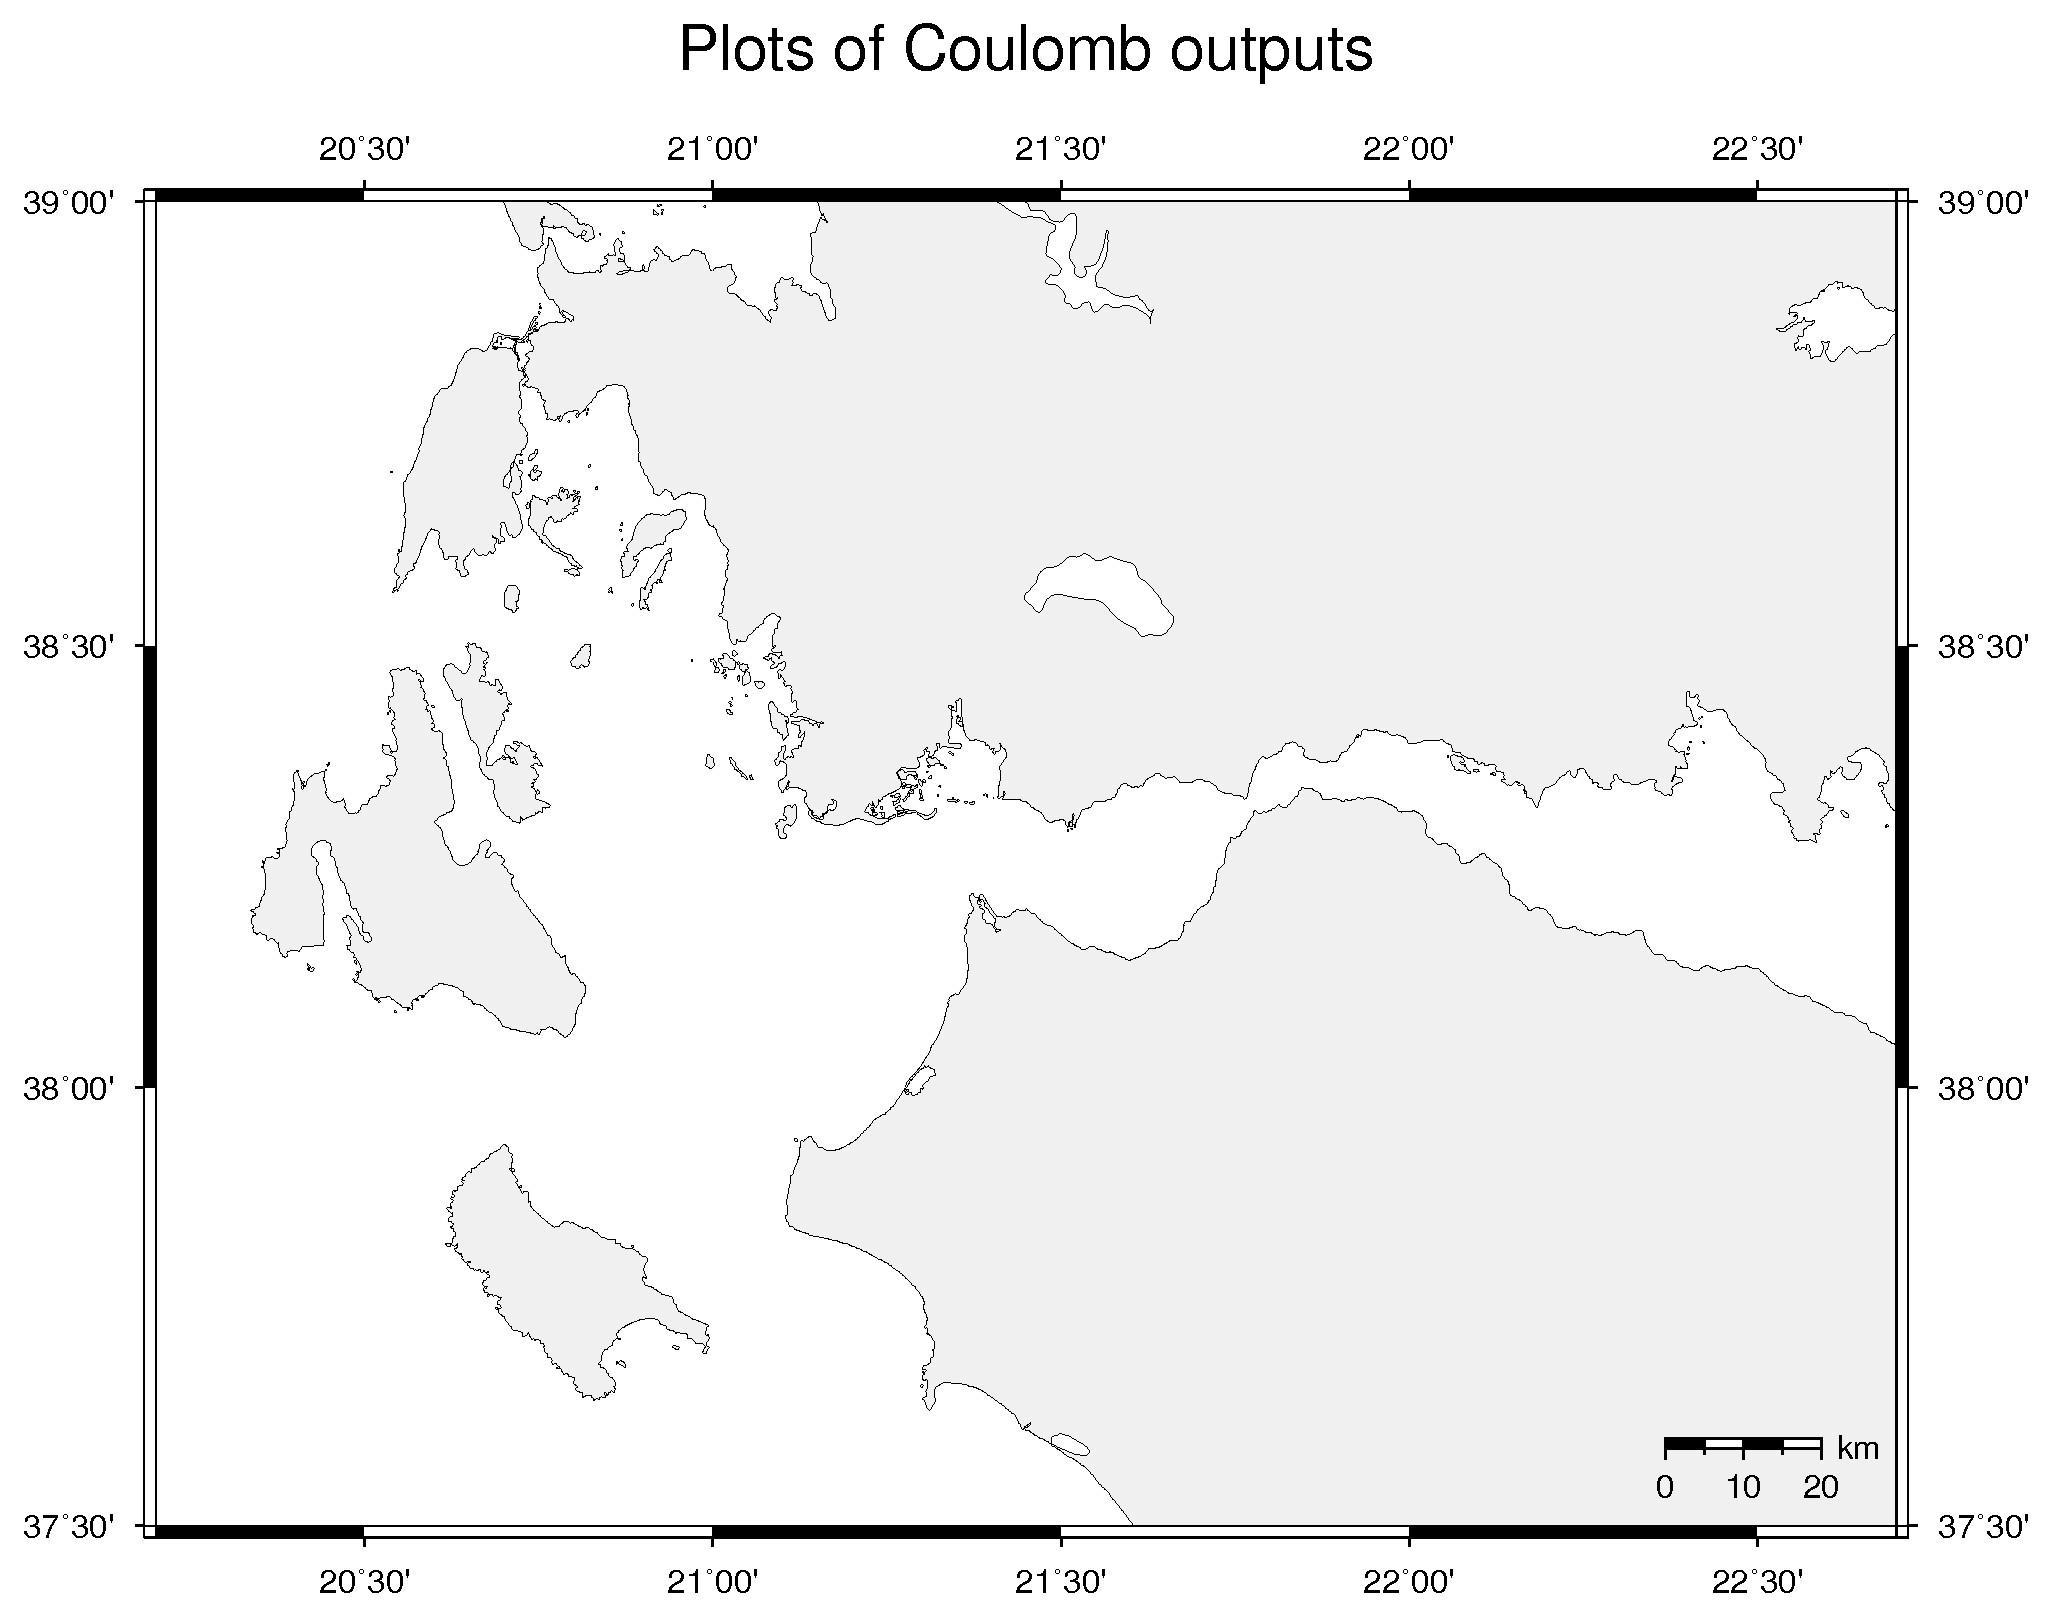
\includegraphics[width=.95\linewidth]{example401.jpg}
  \end{column}
  \begin{column}{.5\textwidth}
  \begin{scriptsize}
\begin{verbnobox}[\vbdelim]
\$ ./coulomb2gmt.sh kef_1953 kef_1953_kef \
                   -outjpg -o example402 \
                   <[red]-r 20.1 20.2 31.2 35.2 1000000>
\end{verbnobox}
\end{scriptsize}
\centering
  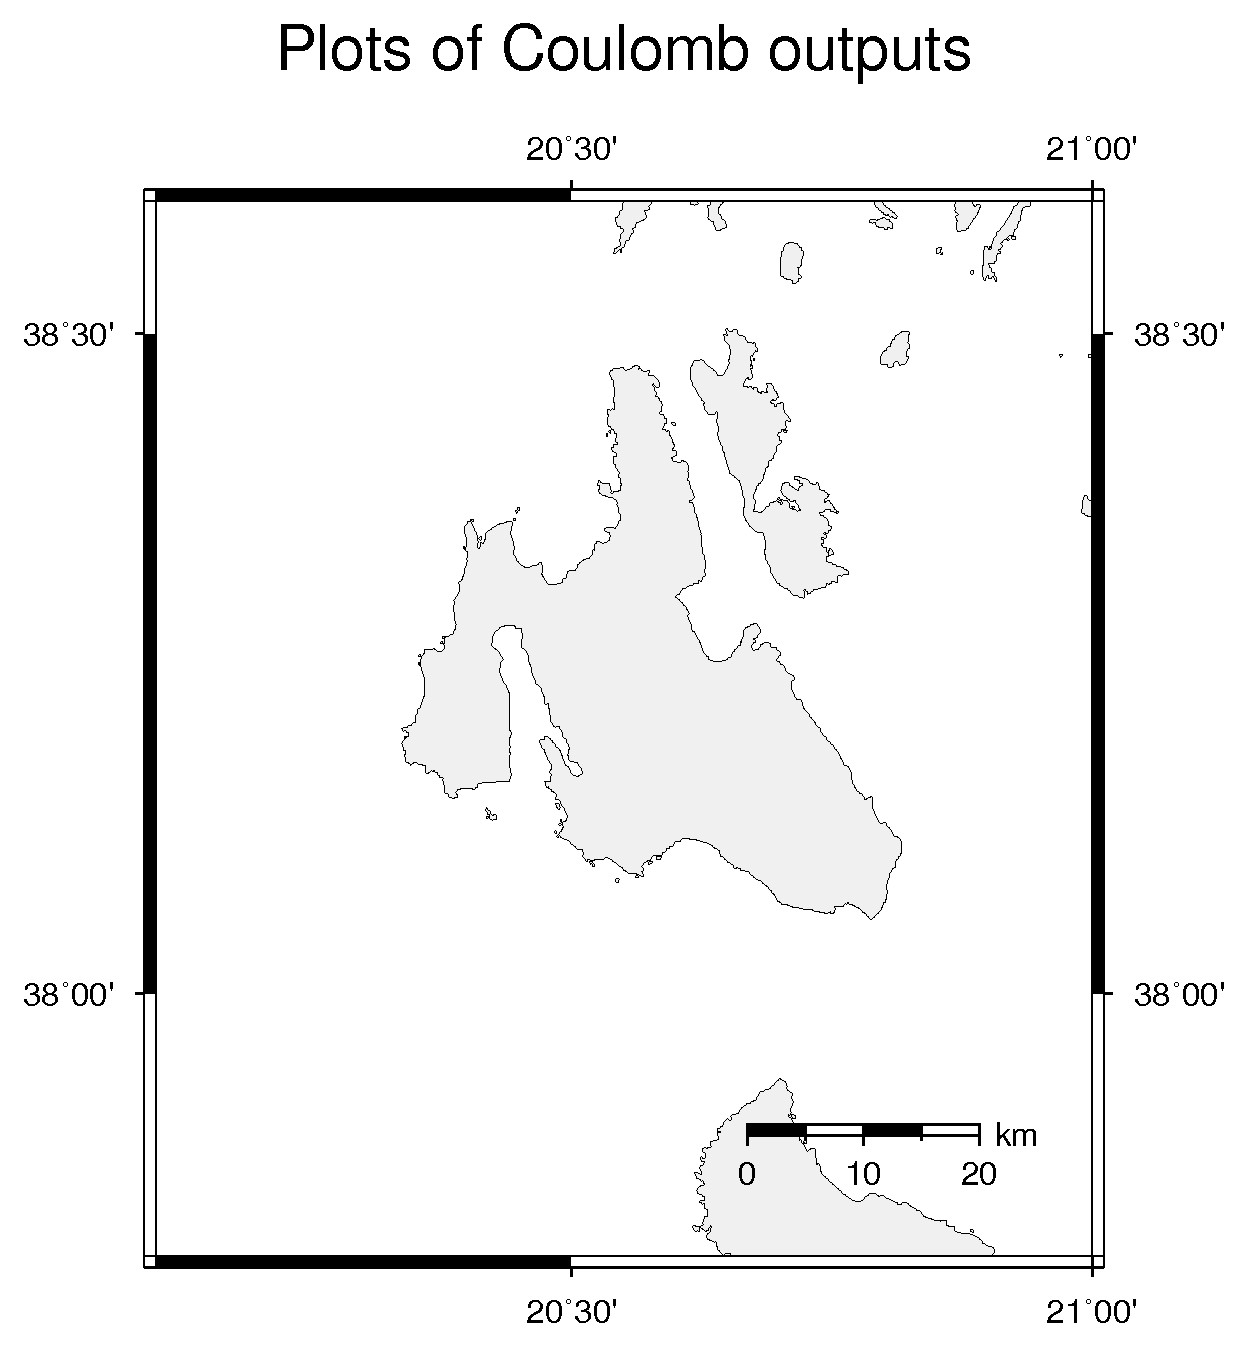
\includegraphics[width=.65\linewidth]{example402.jpg}
  \end{column}
\end{columns}

\end{frame}
\note{}

% //////////////////////////////////////////////////////////////////////////////
\begin{frame}[t,fragile]
  \frametitle{General Options - Examples}
  \framesubtitle{}
  \label{ch4fr:ex403_4}
  \vskip-.6cm
\begin{columns}[t]
  \begin{column}{.5\textwidth}
\begin{scriptsize}
\begin{verbnobox}[\vbdelim]
\$ ./coulomb2gmt.sh kef_1953 kef_1953_kef \
                   -outjpg -o example403 \
                   <[red]-t>
\end{verbnobox}
\end{scriptsize}
\centering
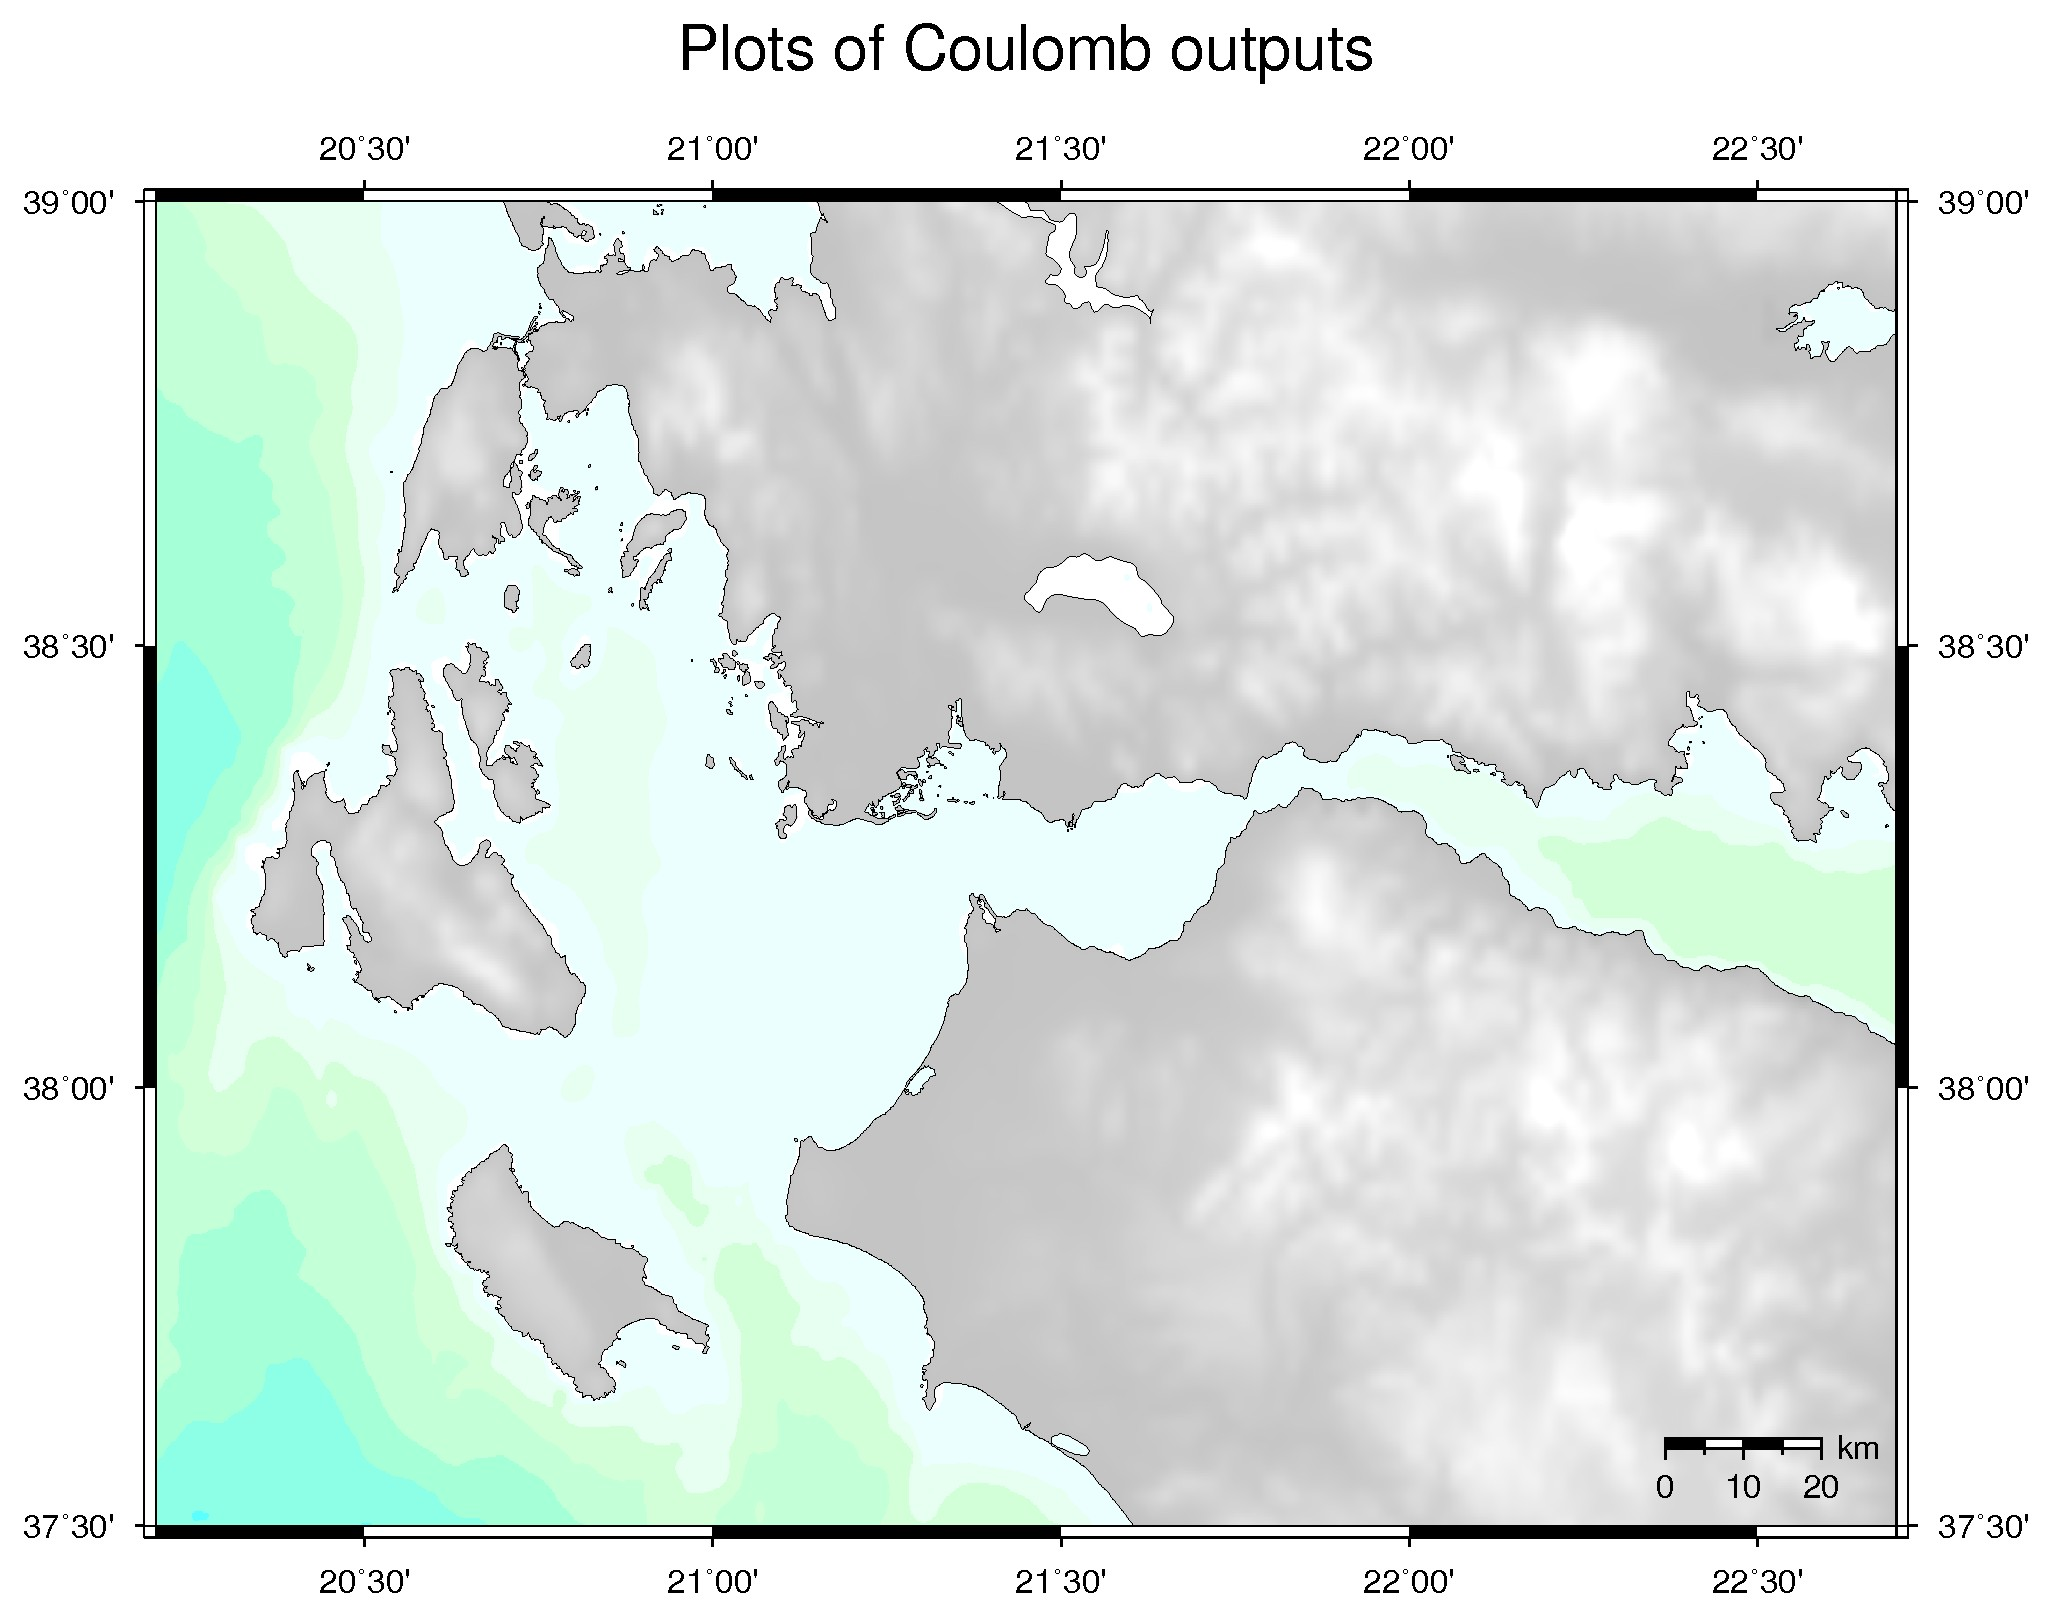
\includegraphics[width=.95\linewidth]{example403.jpg}
  \end{column}
  \begin{column}{.5\textwidth}
  \begin{scriptsize}
\begin{verbnobox}[\vbdelim]
\$ ./coulomb2gmt.sh kef_1953 kef_1953_kef \
                   -outjpg -o example404 \
                   -t <[red]-lg -lc>
\end{verbnobox}
\end{scriptsize}
\centering
  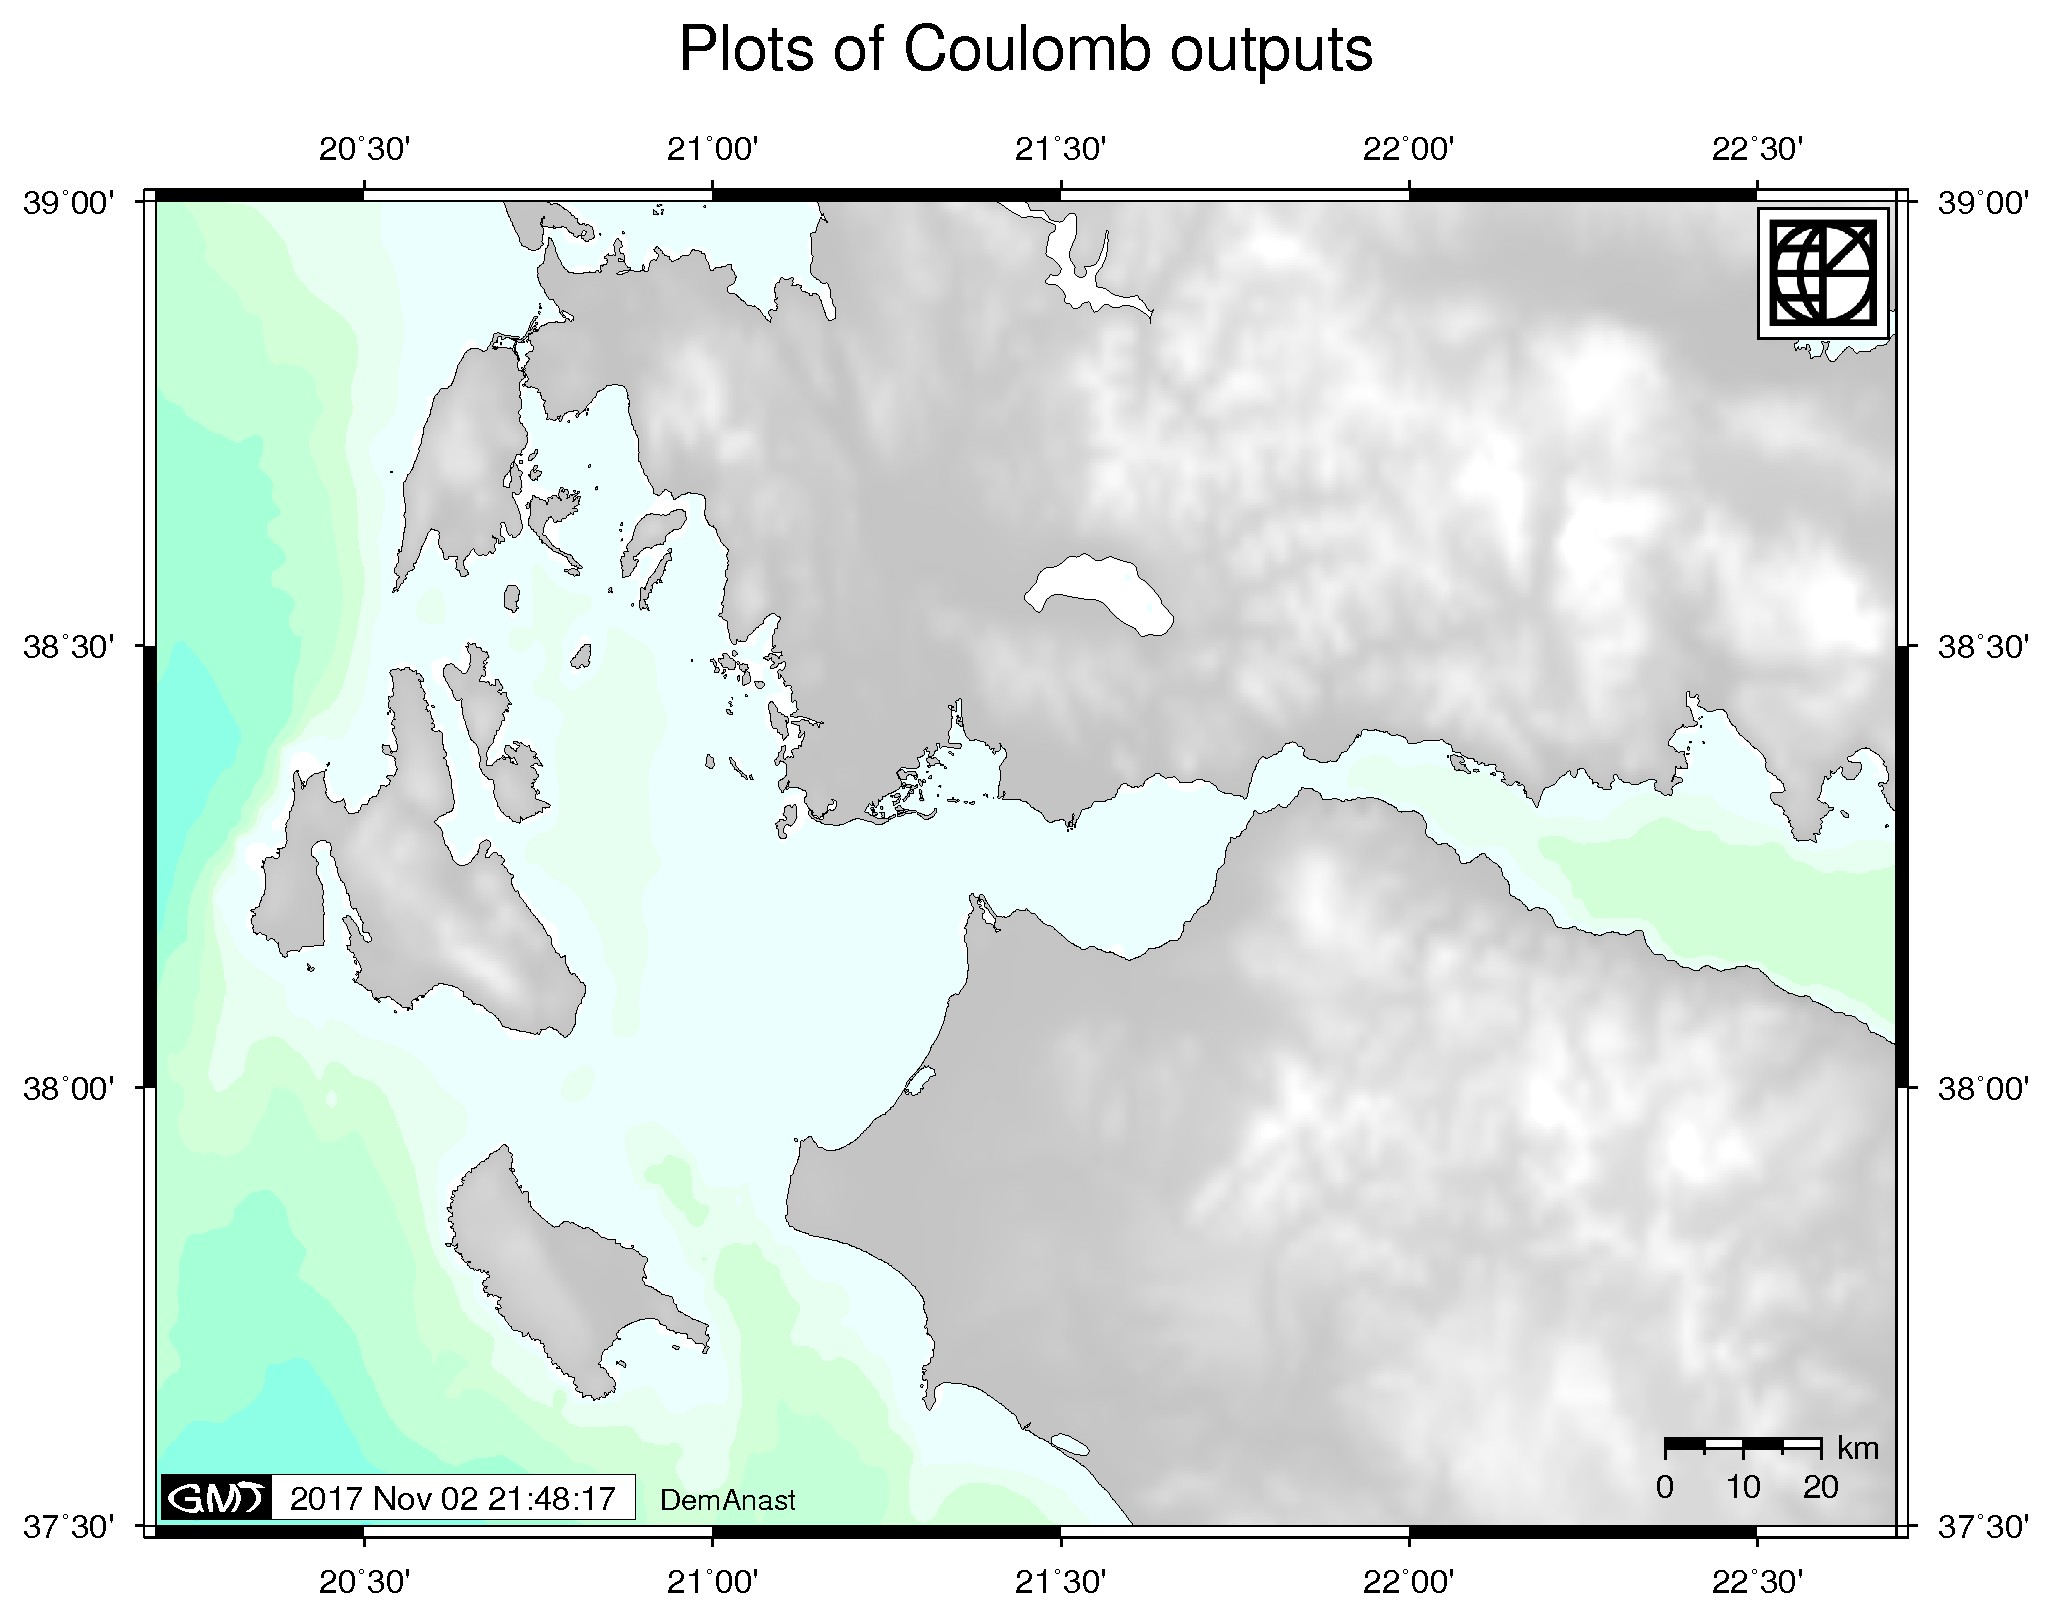
\includegraphics[width=.95\linewidth]{example404.jpg}
  \end{column}
\end{columns}

\end{frame}
\note{}

% //////////////////////////////////////////////////////////////////////////////
\begin{frame}[t,fragile]
  \frametitle{General Options - Examples}
  \framesubtitle{}
  \label{ch4fr:405_6}
    \vskip-.6cm
\begin{columns}[t]
  \begin{column}{.5\textwidth}
\begin{scriptsize}
\begin{verbnobox}[\vbdelim]
\$ ./coulomb2gmt.sh kef_1953 kef_1953_kef \
                   -outjpg -o example405 \
                   -t -lg -lc \
                   <[red]-fproj -fsurf -fdep>
\end{verbnobox}
\end{scriptsize}
\centering
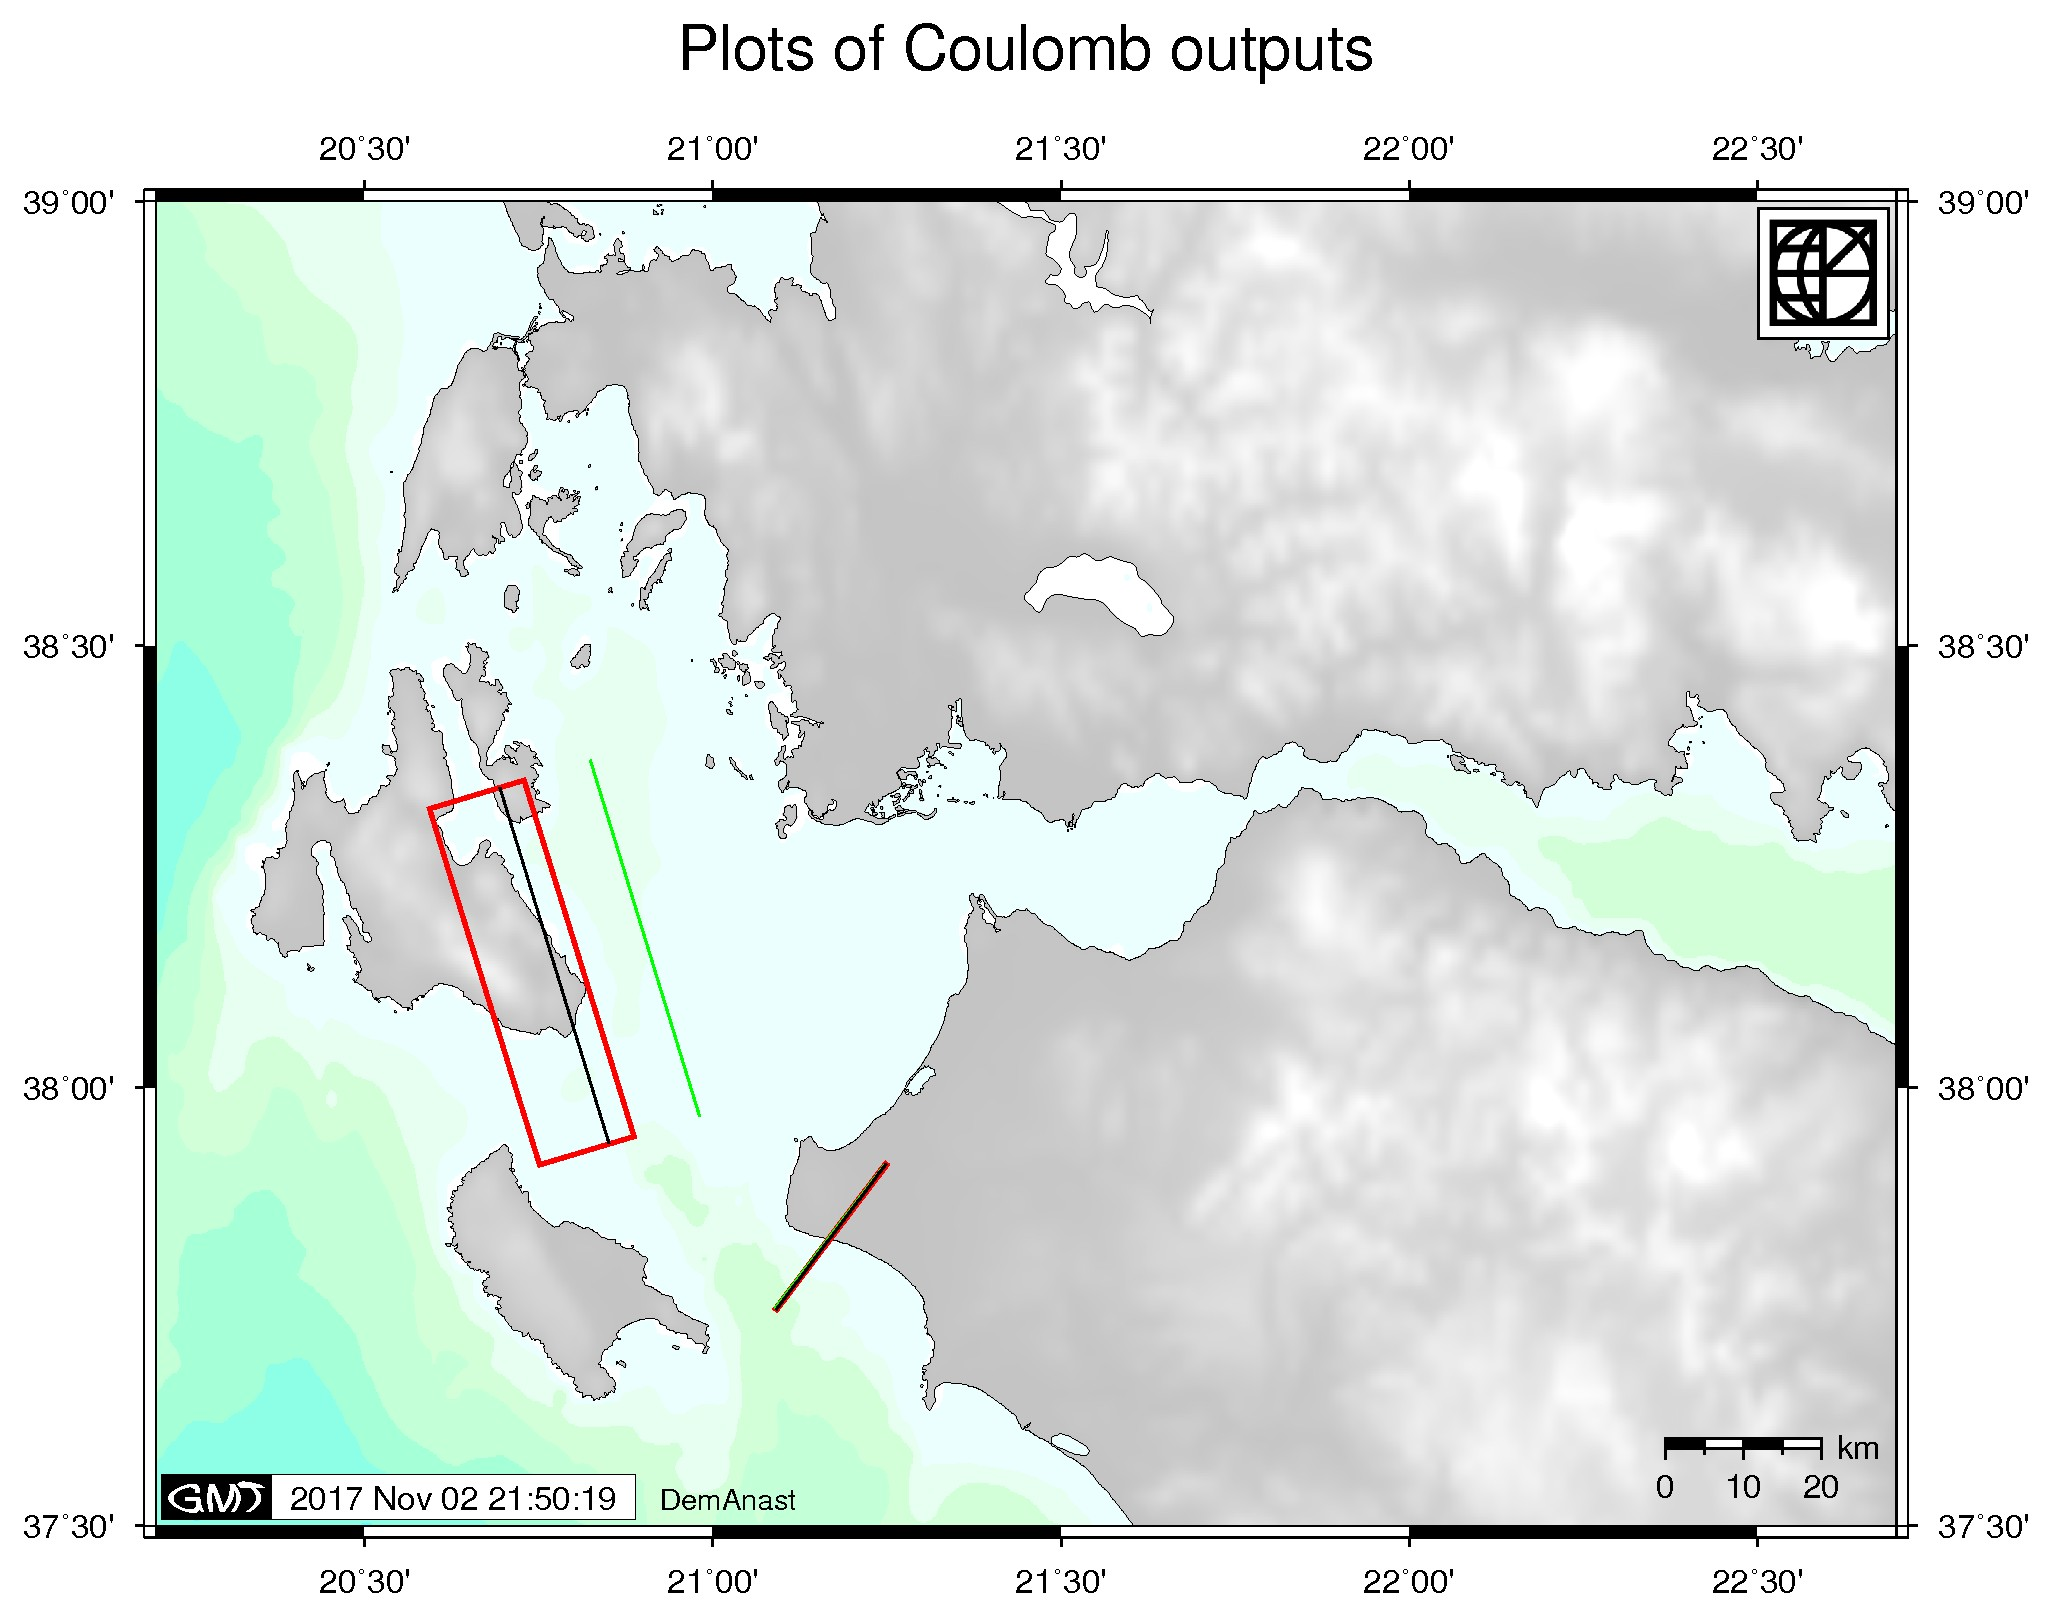
\includegraphics[width=.85\linewidth]{example405.jpg}
  \end{column}
  \begin{column}{.5\textwidth}
  \begin{scriptsize}
\begin{verbnobox}[\vbdelim]
\$ ./coulomb2gmt.sh kef_1953 kef_1953_kef \
                   -outjpg -o example406 \
                   -t -lg -lc \
                   -fproj -fsurf -fdep \
                   <[red]-cmt historic.cmt>
\end{verbnobox}
\end{scriptsize}
\centering
  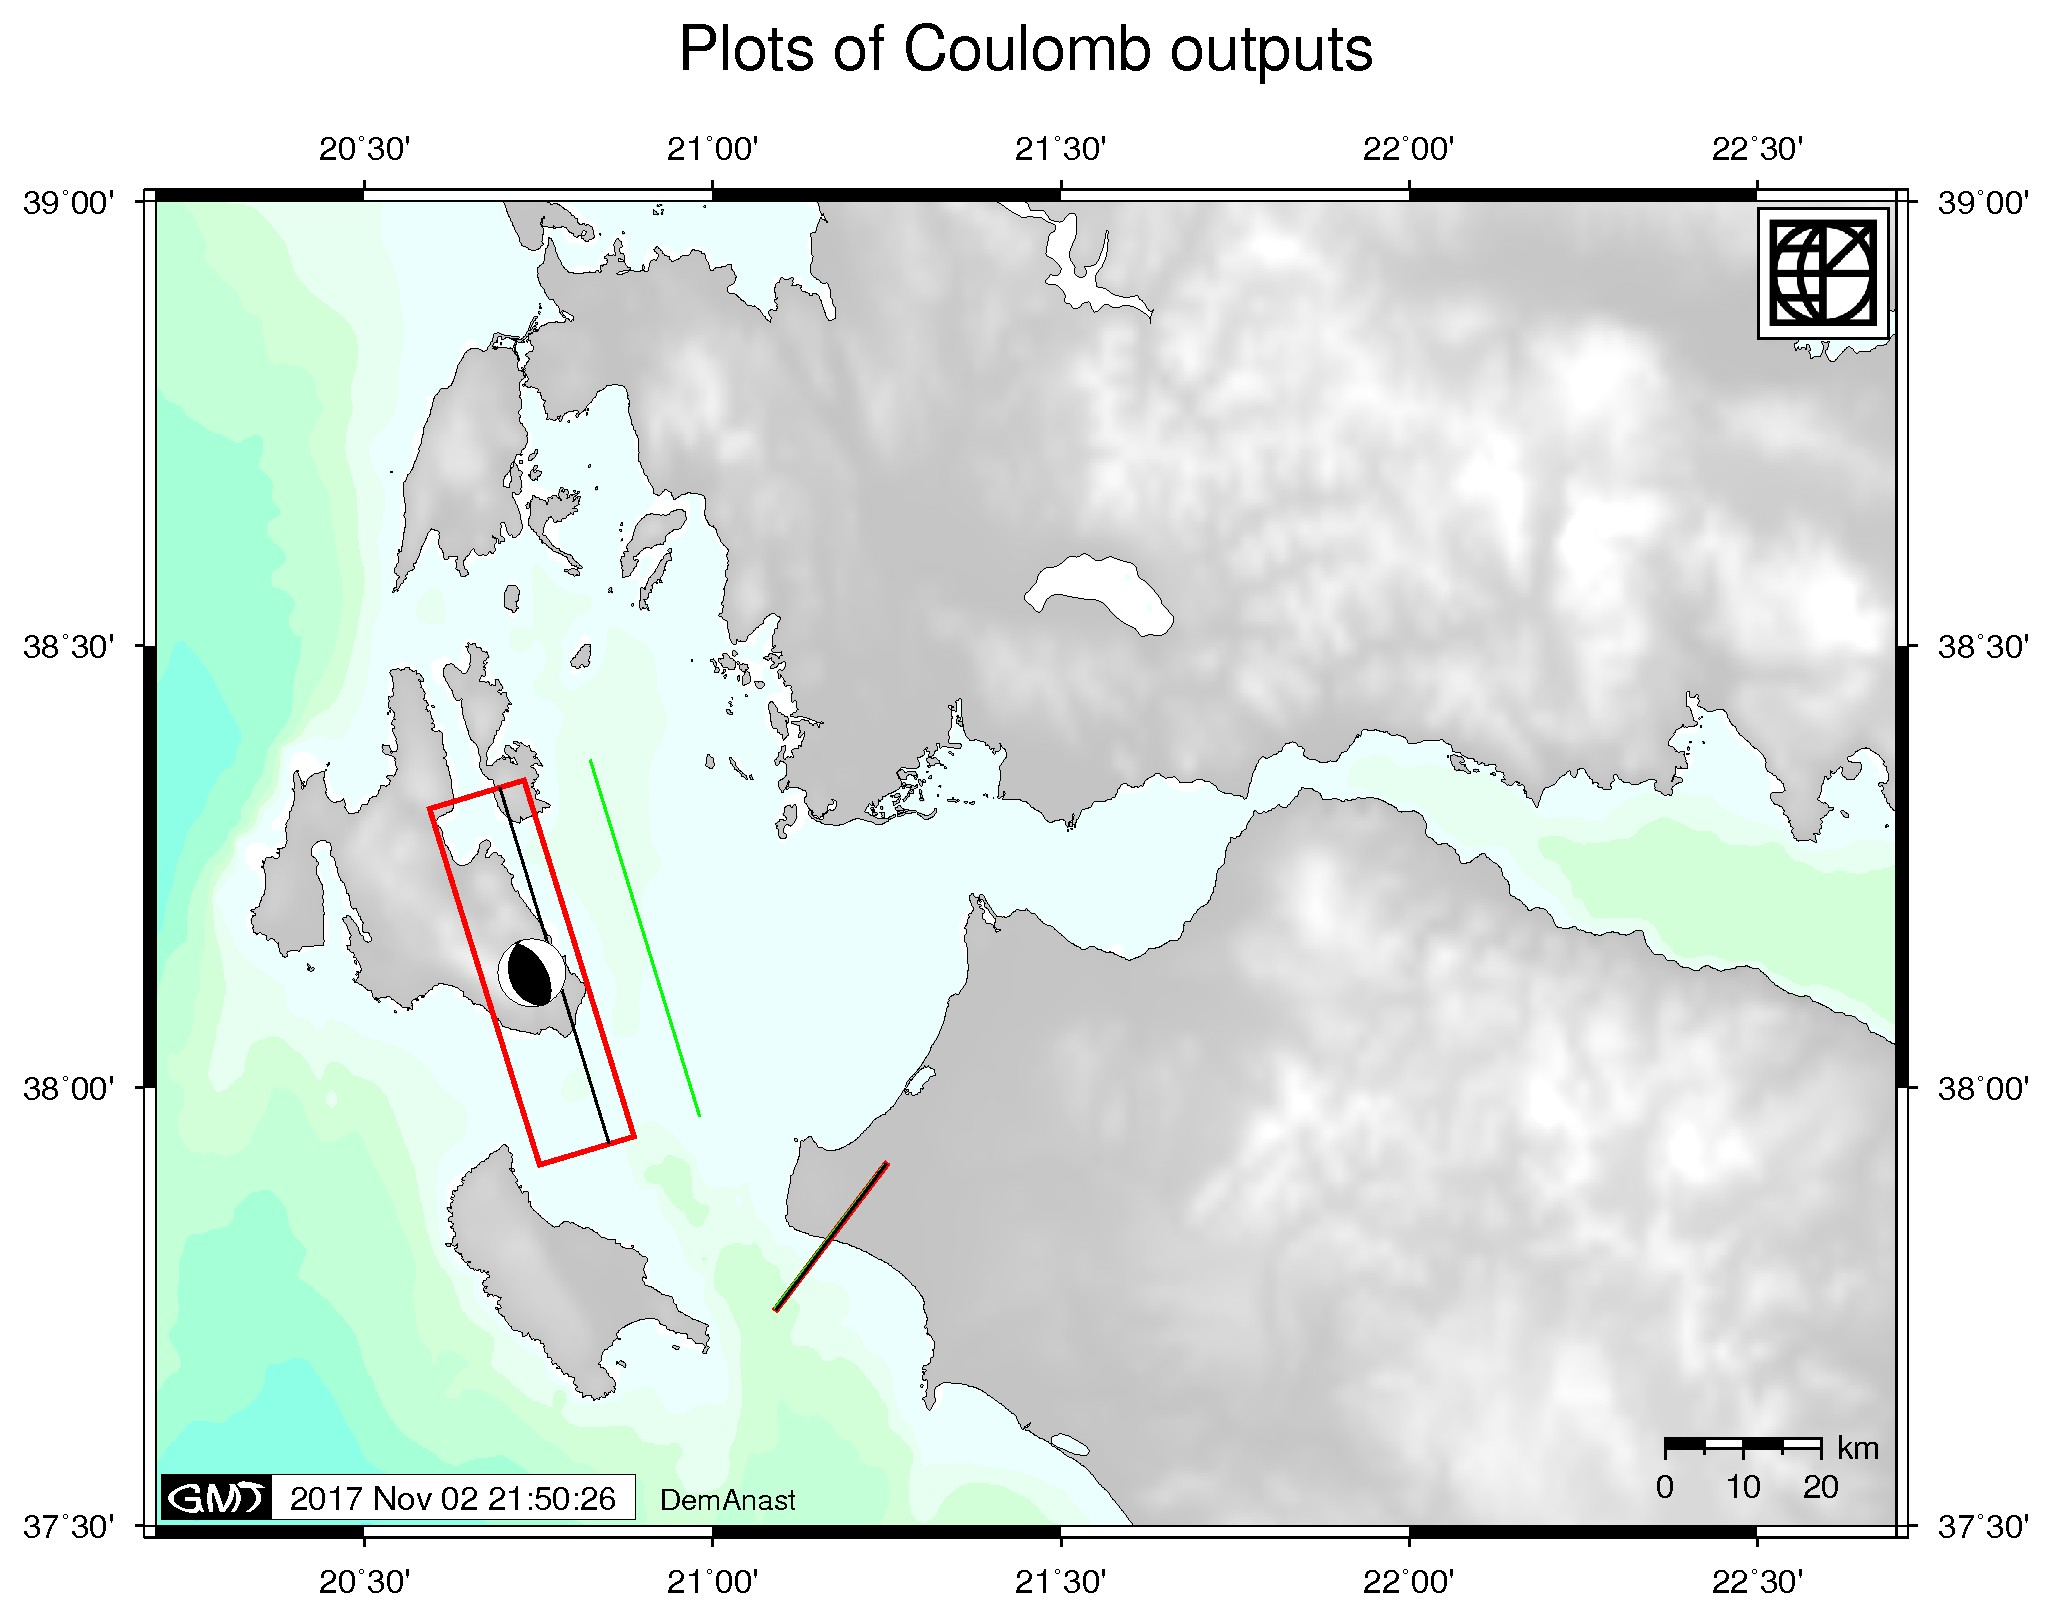
\includegraphics[width=.75\linewidth]{example406.jpg}
  \end{column}
\end{columns}

\end{frame}
\note{}

% //////////////////////////////////////////////////////////////////////////////
\begin{frame}[t,fragile]
  \frametitle{General Options - Examples}
  \framesubtitle{}
  \label{ch4fr:ex407}
  \vskip-.6cm
\begin{columns}[t]
  \begin{column}{.5\textwidth}
\begin{scriptsize}
\begin{verbnobox}[\vbdelim]
\$ ./coulomb2gmt.sh kef_1953 kef_1953_kef \
                   -outjpg \ 
                   --output example407 \
                   --topography \
                   --logo_gmt \
                   --logo_custom \
                   --moment_tensor historic.cmt \
                   <[red]--eq_distribution CAT2014.TXT \>
                   <[red]--map_title "Example 407" \>
                   -fproj \
                   -fsurf \
                   -fdep
\end{verbnobox}
\end{scriptsize}

  \end{column}
  \begin{column}{.5\textwidth}

\centering
  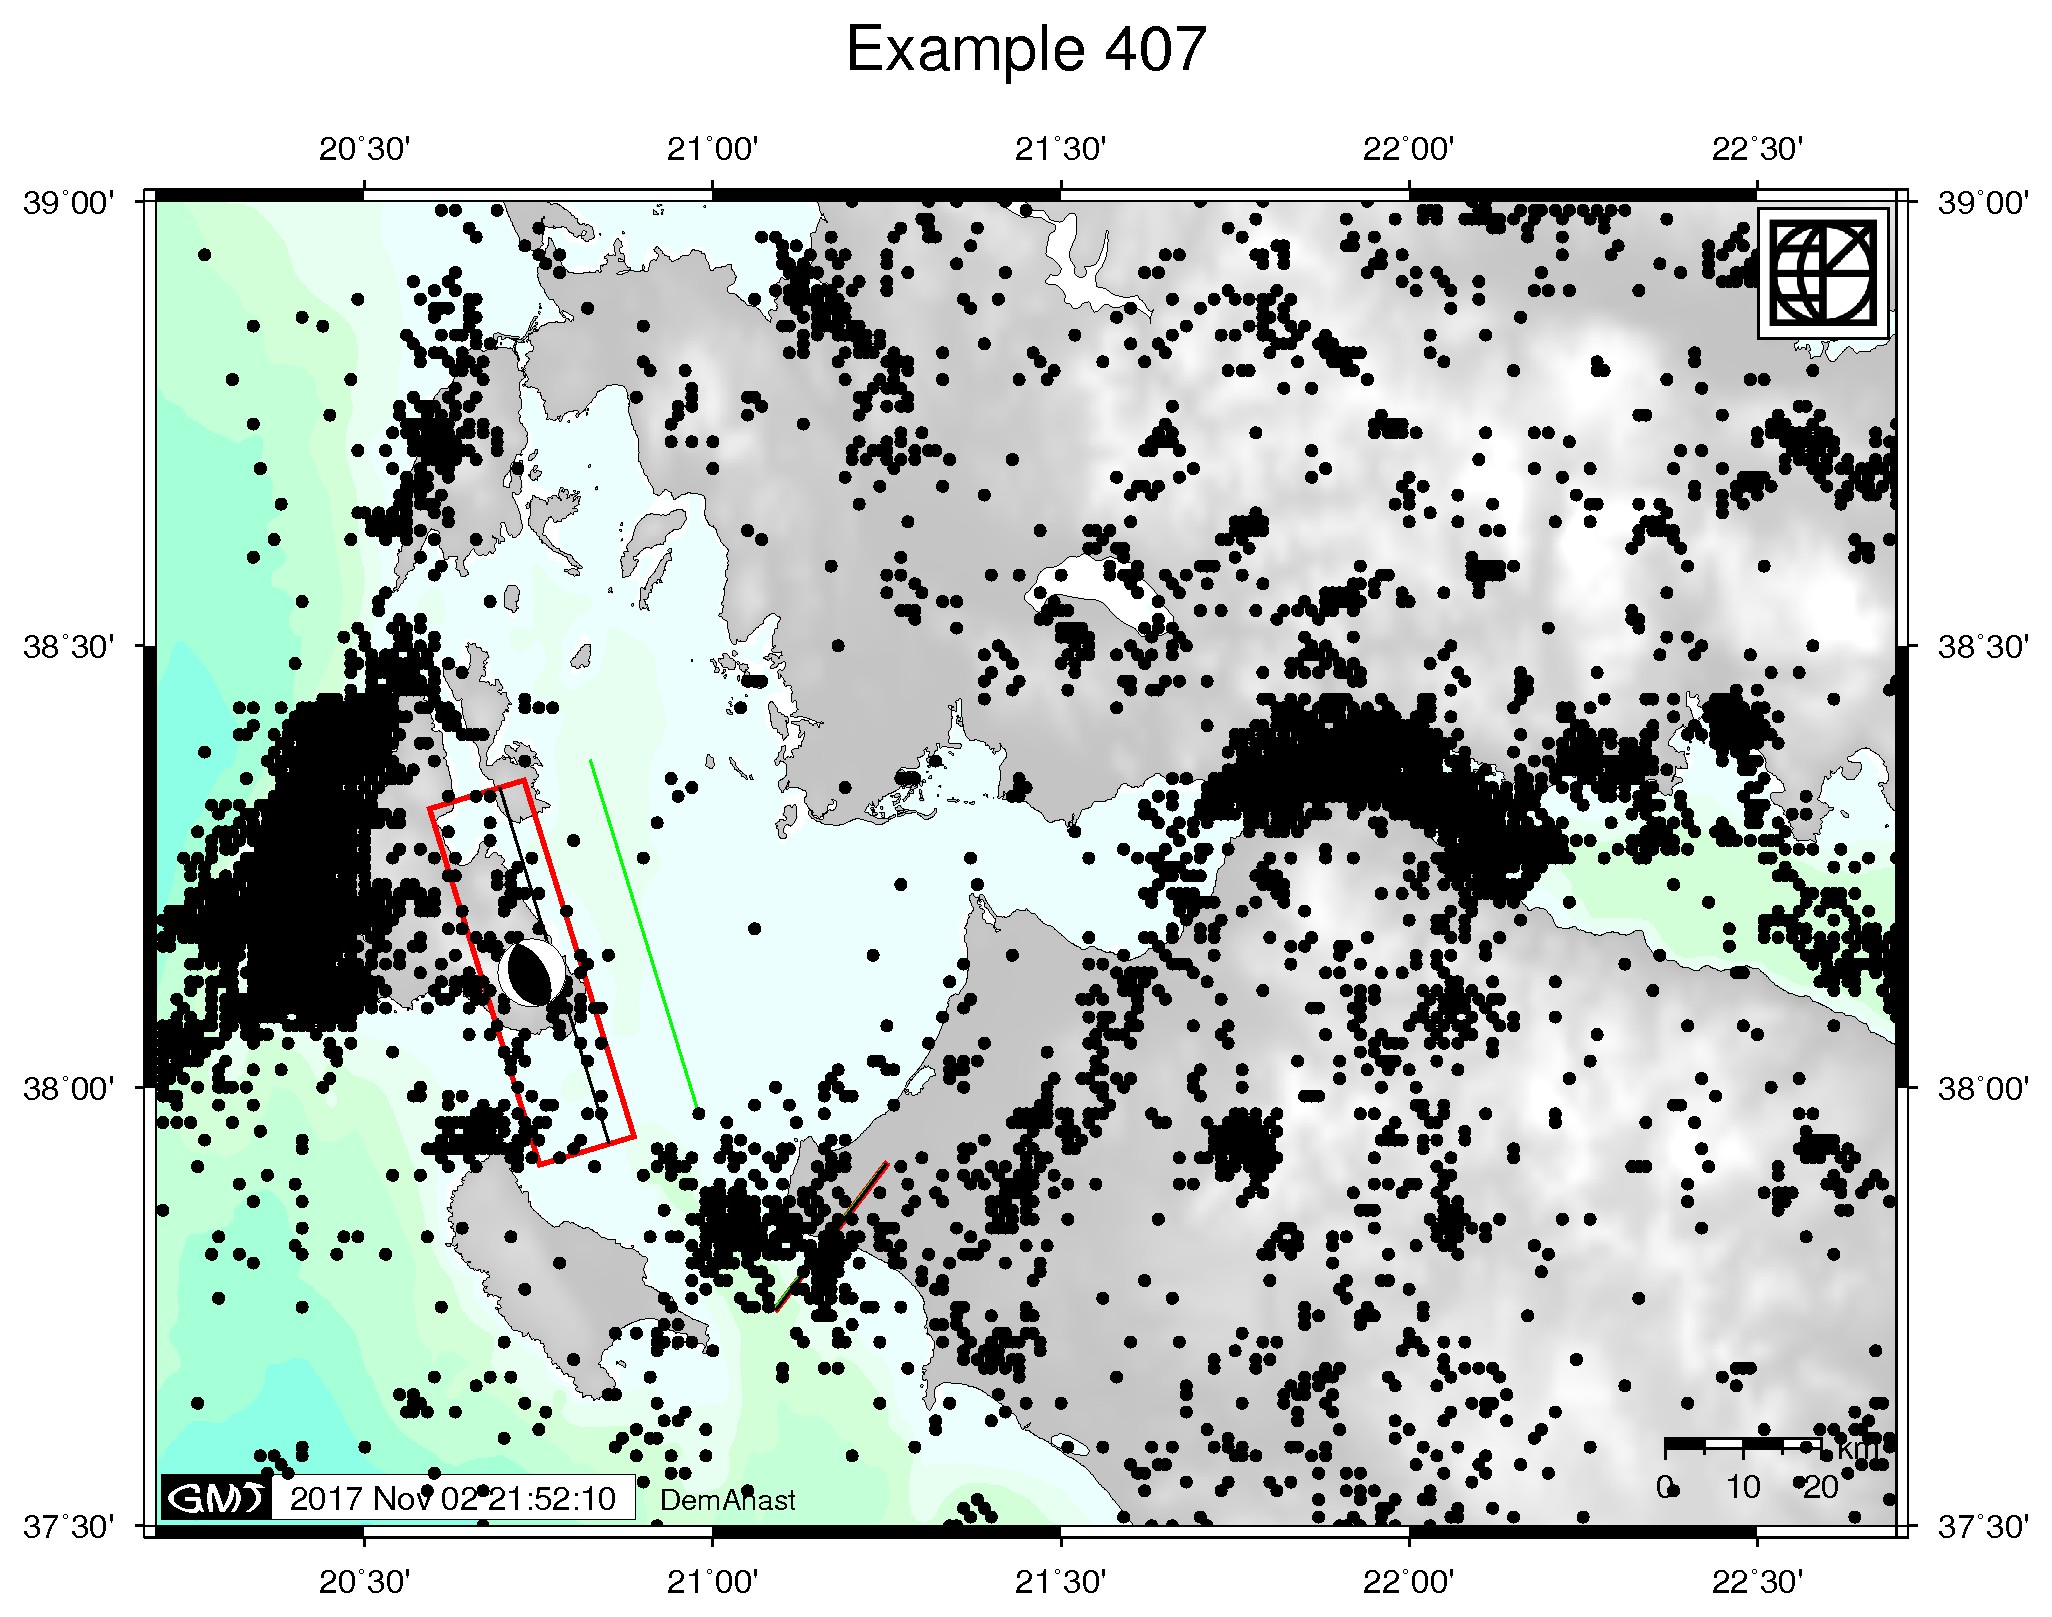
\includegraphics[width=.95\linewidth]{example407.jpg}
  \end{column}
\end{columns}

\end{frame}
\note{}

% //////////////////////////////////////////////////////////////////////////////
\begin{frame}[t,fragile]
  \frametitle{Common mistakes - error messages}
  \framesubtitle{}
  \label{ch4fr:ex408}
  \vskip-.6cm
\begin{columns}[t]
  \begin{column}{.5\textwidth}
\begin{scriptsize}
\begin{verbatim}
$ ./coulomb2gmt.sh kef_1953 kef_1953_kef \

\end{verbatim}
\end{scriptsize}

  \end{column}
  \begin{column}{.5\textwidth}

\centering
%  \includegraphics[width=.95\linewidth]{example408.jpg}
  \end{column}
\end{columns}

\end{frame}
\note{}






















\section[Stress/Strain]{Stress/Strain plots}

\graphicspath{{Chapter5/Figs/}}

% //////////////////////////////////////////////////////////////////////////////
\begin{frame}
  \frametitle{Stress/Strain plots}
  \framesubtitle{}
  \label{ch5fr:stroptions}
\begin{scriptsize}


\emph{Plot stress}

\begin{itemize}
\item
  \texttt{-cstress}: Plot Coulomb Stress change.
\item
  \texttt{-sstress}: Plot Shear Stress change.
\item
  \texttt{-nstress}: Plot Normal Stress change.
\item
  \texttt{-fcross}: Plot cross section of stress change or dilatation.
\end{itemize}

\emph{Plot Strain components}

\begin{itemize}
\item
  \texttt{-stre**}: Where \texttt{**} you can fill all strain components
  \texttt{xx},\texttt{yy},\texttt{zz}, \texttt{yz}, \texttt{xz},
  \texttt{xy}.
\item
  \texttt{-strdil}: Plot dilatation (Exx + Eyy + Ezz )
\end{itemize}

\emph{Overlay Stress/strain on the top of DEM}

\texttt{-****+ot}: use \texttt{+ot} after the main argument to overlay
the raster output on the top of DEM. configure transparency in
\texttt{default-param} file. \textbf{Be careful} transparency can
printed only in JPEG, PNG and PDF outputs.
\end{scriptsize}
\end{frame}
\note{}

% //////////////////////////////////////////////////////////////////////////////
\begin{frame}[t,fragile]
  \frametitle{Coulomb Stress Change}
  \framesubtitle{Example 501}
  \label{ch5fr:ex501}
\begin{columns}[t]
  \begin{column}{.5\textwidth}
\begin{scriptsize}
\begin{verbatim}
$ ./coulomb2gmt.sh kef_1953 kef_1953_kef \
                   -outjpg \ 
                   --output example501 \
                   --logo_gmt \
                   --moment_tensor historic.cmt \
                   -fproj \
                   -fsurf \
                   -fdep \
                   -cstress
\end{verbatim}
\end{scriptsize}

  \end{column}
  \begin{column}{.5\textwidth}

\centering
  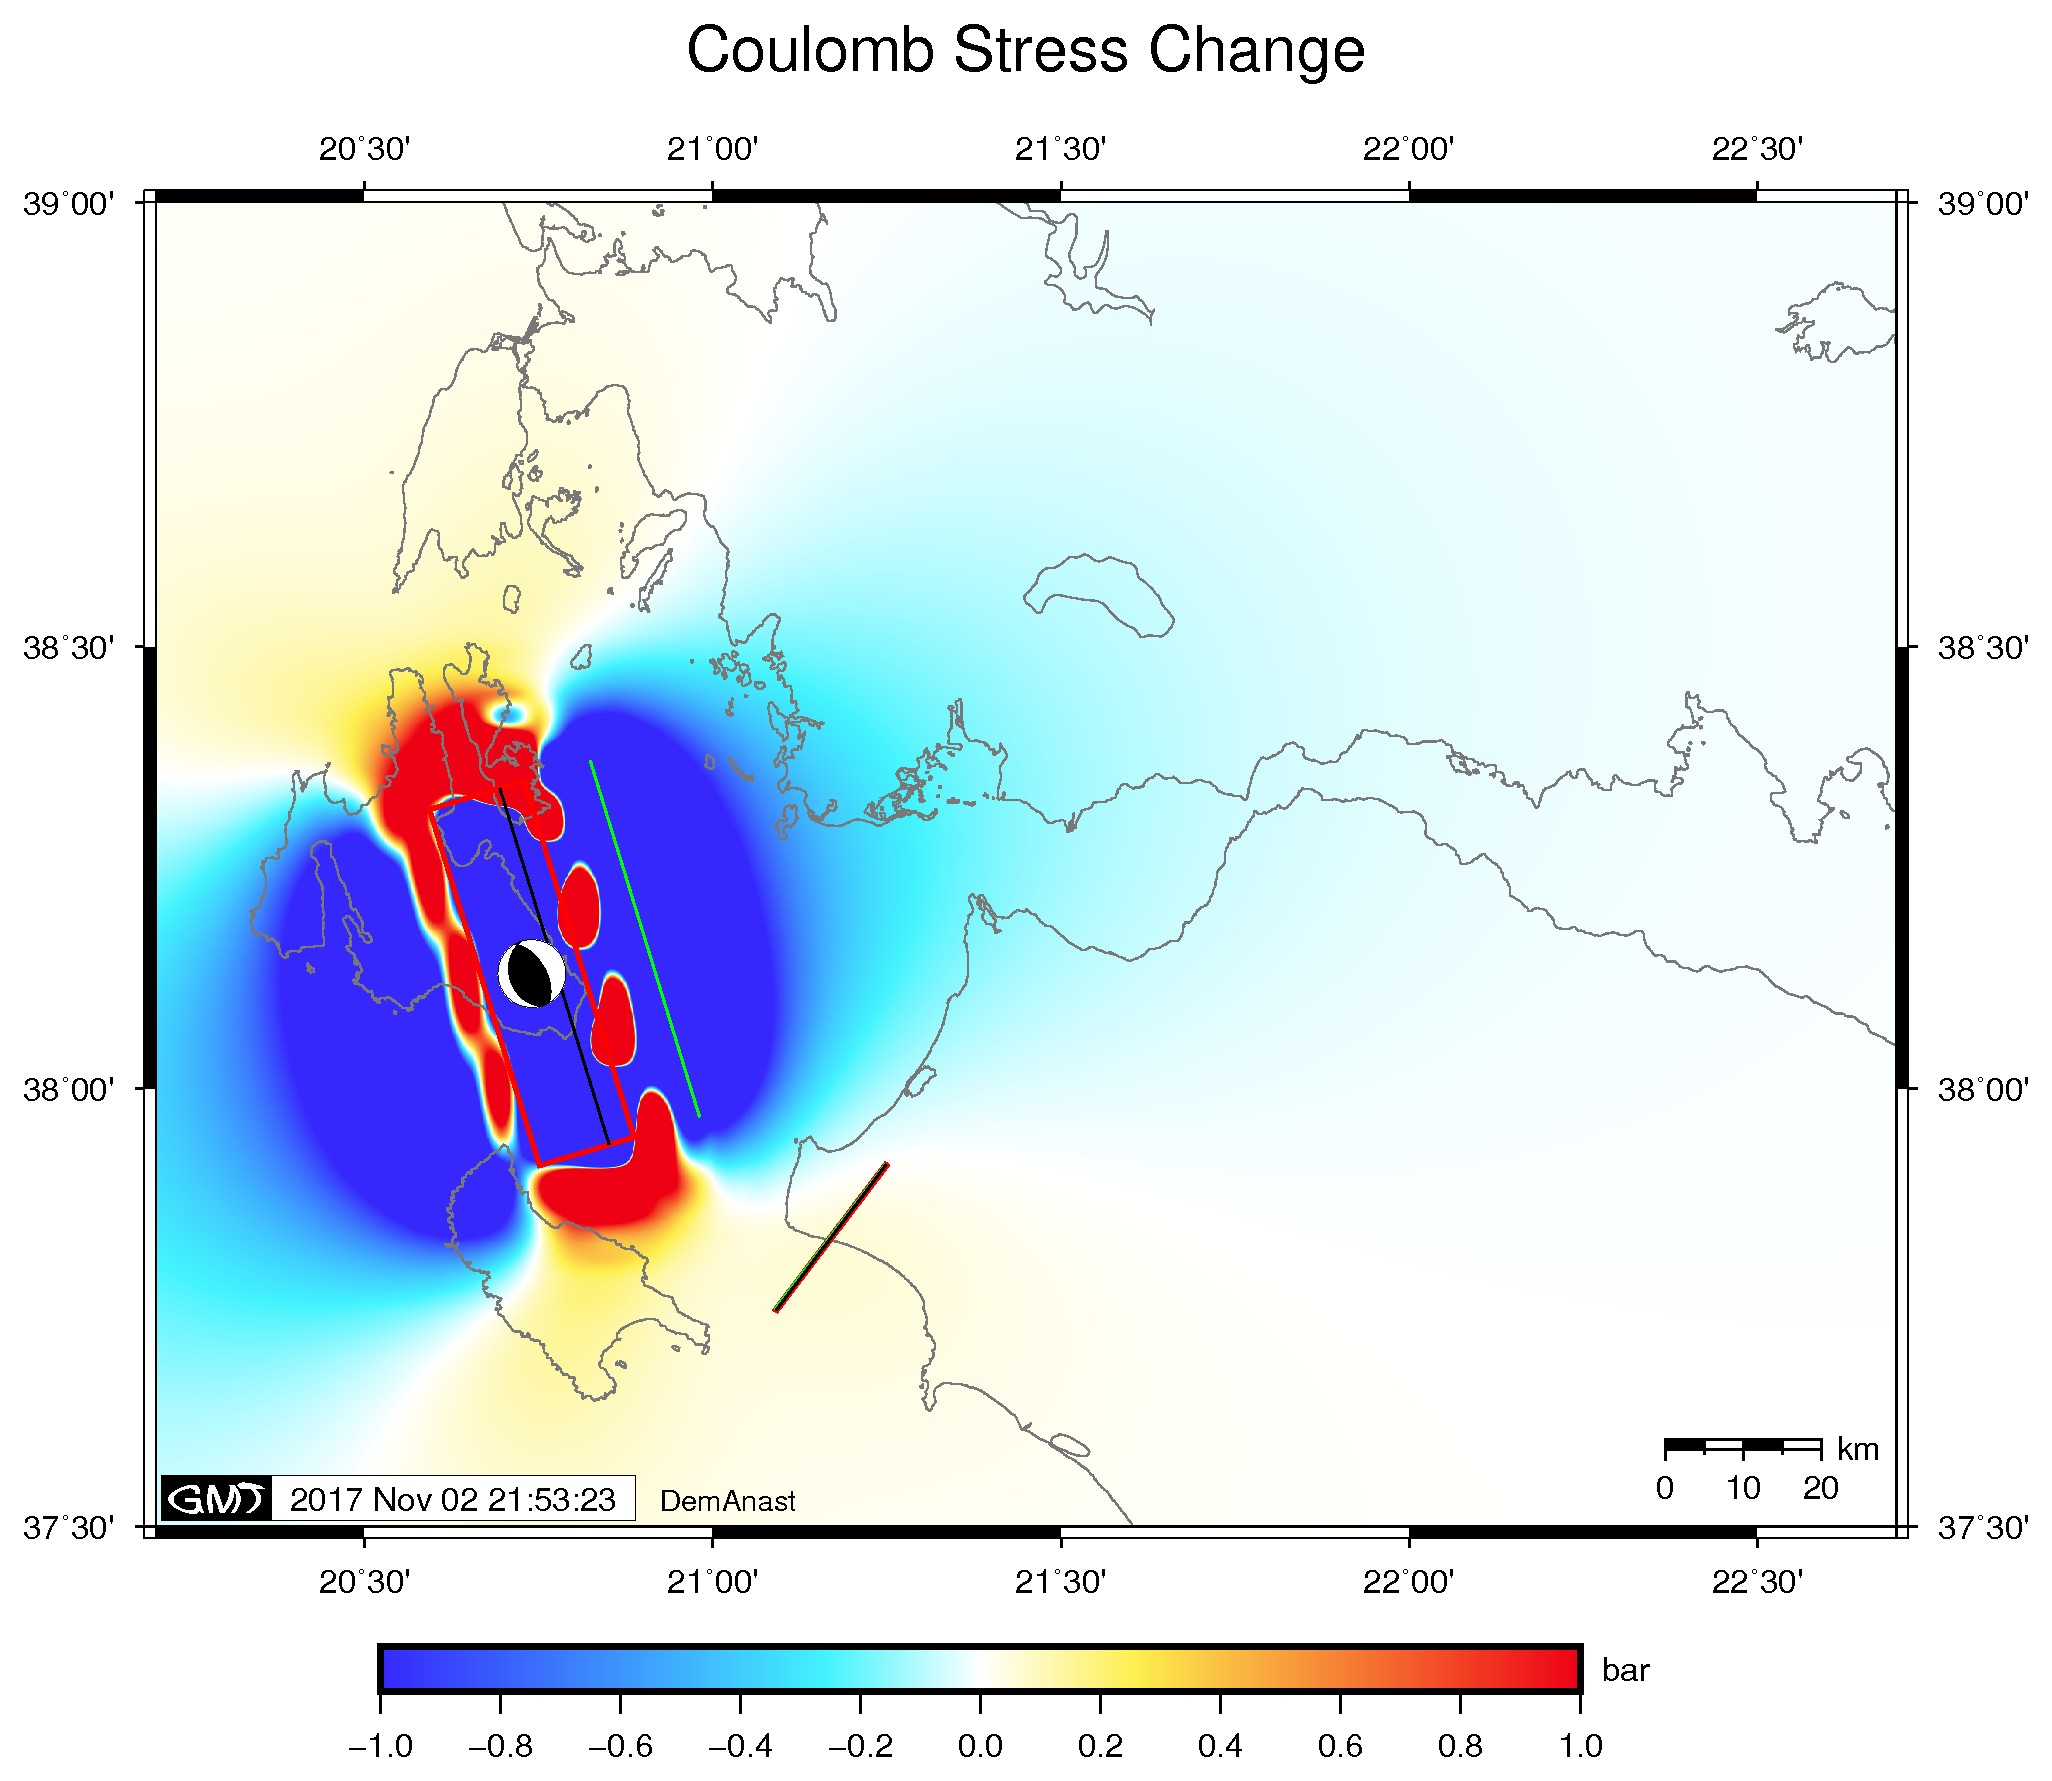
\includegraphics[width=.95\linewidth]{example501.jpg}
  \end{column}
\end{columns}

\end{frame}
\note{}

% //////////////////////////////////////////////////////////////////////////////
\begin{frame}[t,fragile]
  \frametitle{Coulomb Stress Change overlay topography}
  \framesubtitle{Example 502}
  \label{ch5fr:ex502}
\begin{columns}[t]
  \begin{column}{.5\textwidth}
\begin{scriptsize}
\begin{verbatim}
$ ./coulomb2gmt.sh kef_1953 kef_1953_kef \
                   -outjpg \ 
                   --output example502 \
                   --logo_gmt \
                   --moment_tensor historic.cmt \
                   -fproj \
                   -fsurf \
                   -fdep \
                   -cstress+ot
\end{verbatim}
\end{scriptsize}

  \end{column}
  \begin{column}{.5\textwidth}

\centering
  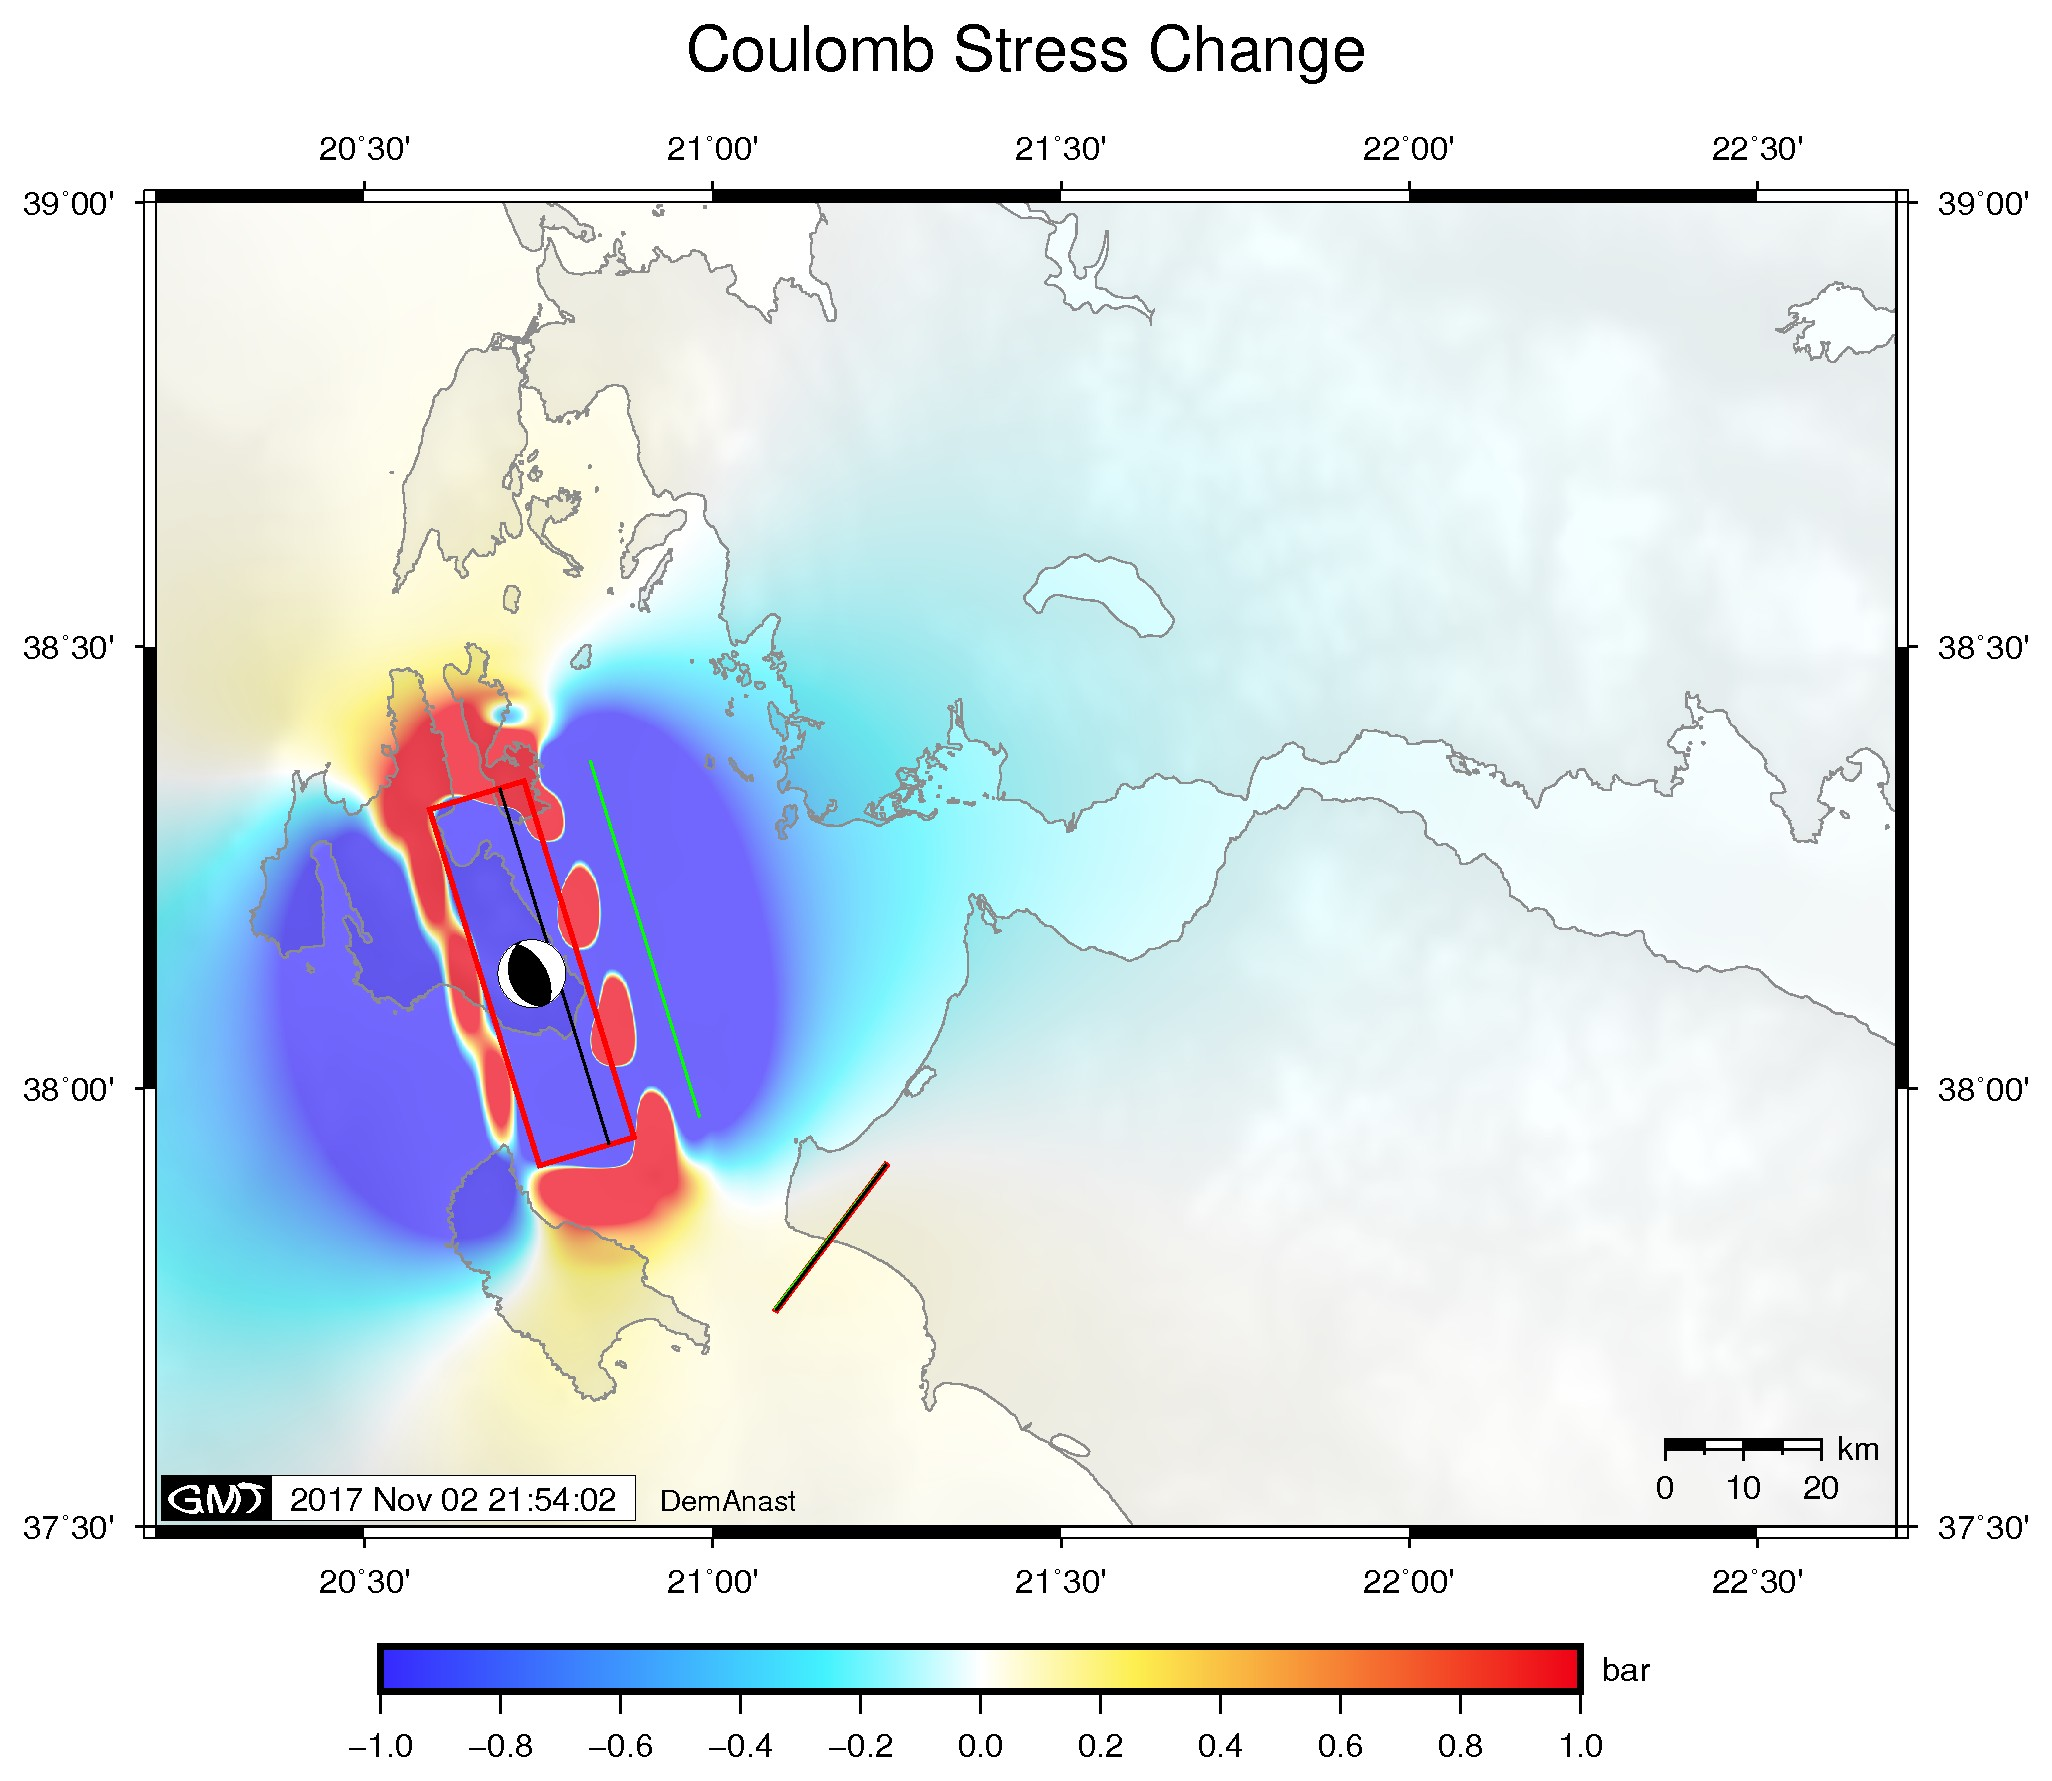
\includegraphics[width=.95\linewidth]{example502.jpg}
  \end{column}
\end{columns}

\end{frame}
\note{}

% //////////////////////////////////////////////////////////////////////////////
\begin{frame}[t,fragile]
  \frametitle{Coulomb Stress Change overlay topography and Cross Section}
  \framesubtitle{Example 503}
  \label{ch5fr:ex503}
\begin{columns}[t]
  \begin{column}{.5\textwidth}
\begin{scriptsize}
\begin{verbatim}
$ ./coulomb2gmt.sh kef_1953 kef_1953_kef \
                   -outjpg \ 
                   --output example503 \
                   --logo_gmt \
                   --moment_tensor historic.cmt \
                   -fproj \
                   -fsurf \
                   -fdep \
                   -cstress+ot \ 
                   -fcross
\end{verbatim}
\end{scriptsize}

  \end{column}
  \begin{column}{.5\textwidth}

\centering
  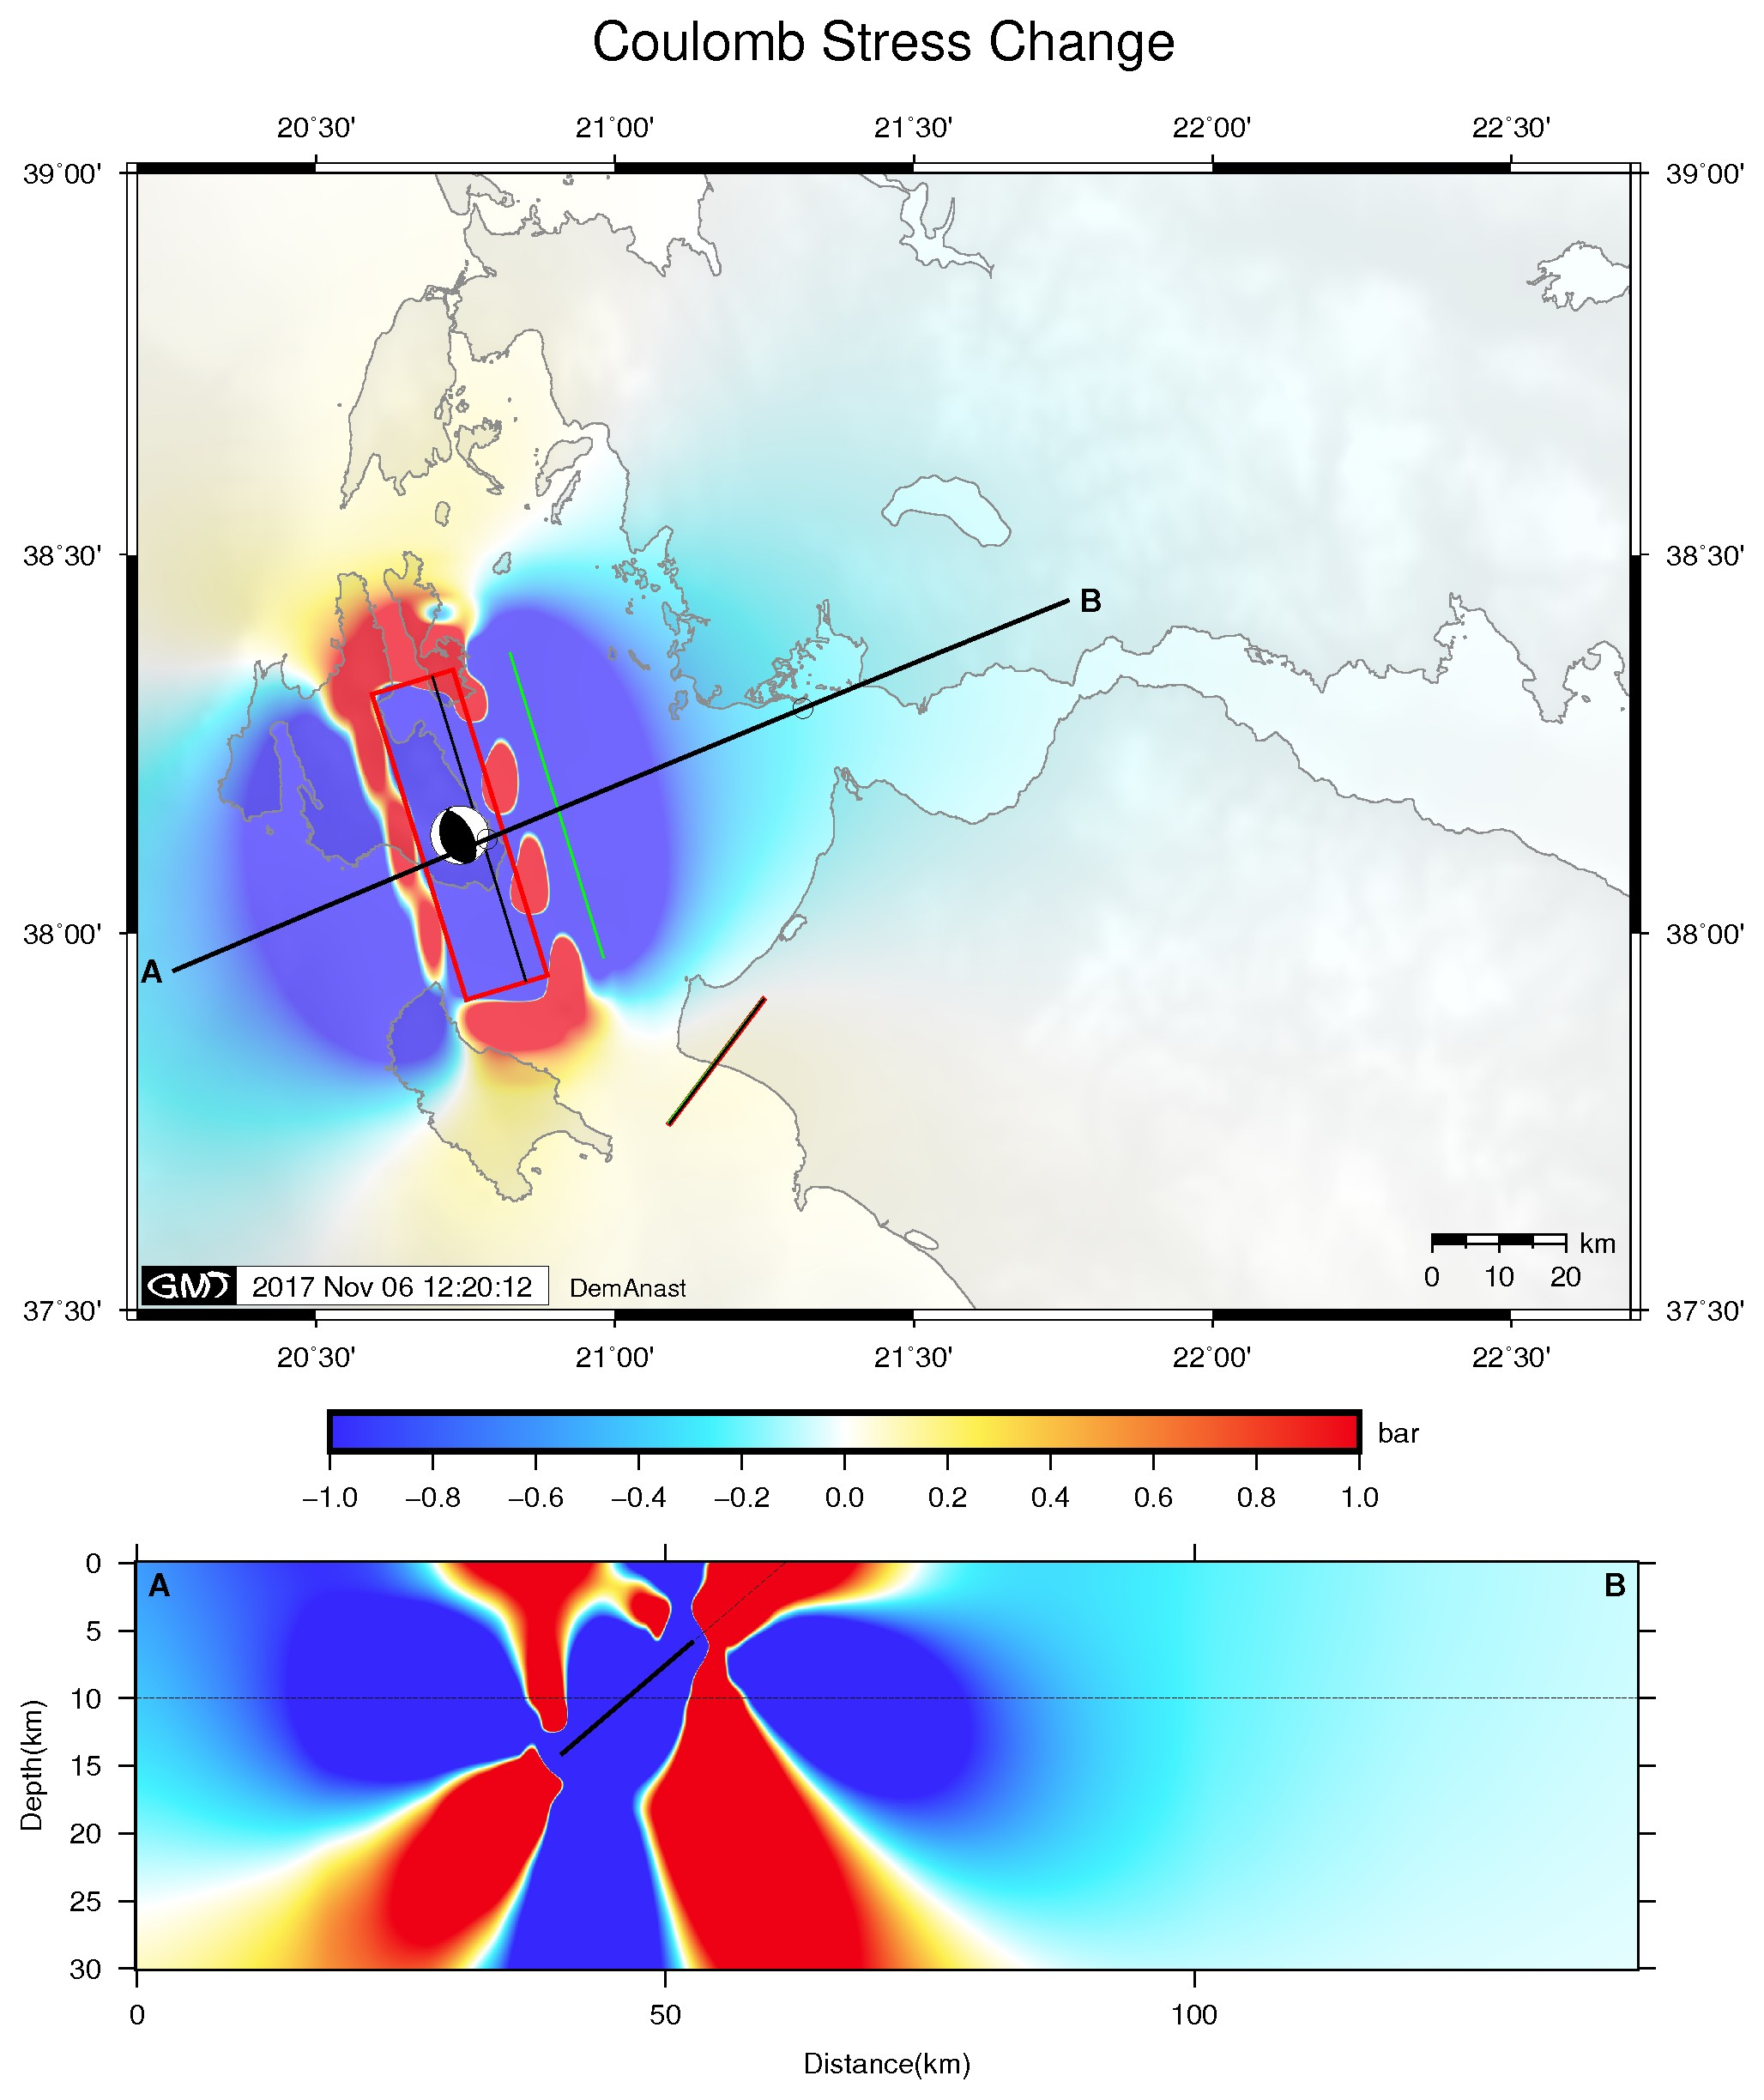
\includegraphics[width=.75\linewidth]{example503.jpg}
  \end{column}
\end{columns}

\end{frame}
\note{}

% //////////////////////////////////////////////////////////////////////////////
\begin{frame}[t,fragile]
  \frametitle{Strain Component Eyy}
  \framesubtitle{Example 504}
  \label{ch5fr:ex504}
\begin{columns}[t]
  \begin{column}{.5\textwidth}
\begin{scriptsize}
\begin{verbatim}
$ ./coulomb2gmt.sh kef_1953 kef_1953_kef \
                   -outjpg \ 
                   --output example504 \
                   --logo_gmt \
                   --moment_tensor historic.cmt \
                   -fproj \
                   -fsurf \
                   -fdep \
                   -streyy
\end{verbatim}
\end{scriptsize}

  \end{column}
  \begin{column}{.5\textwidth}

\centering
  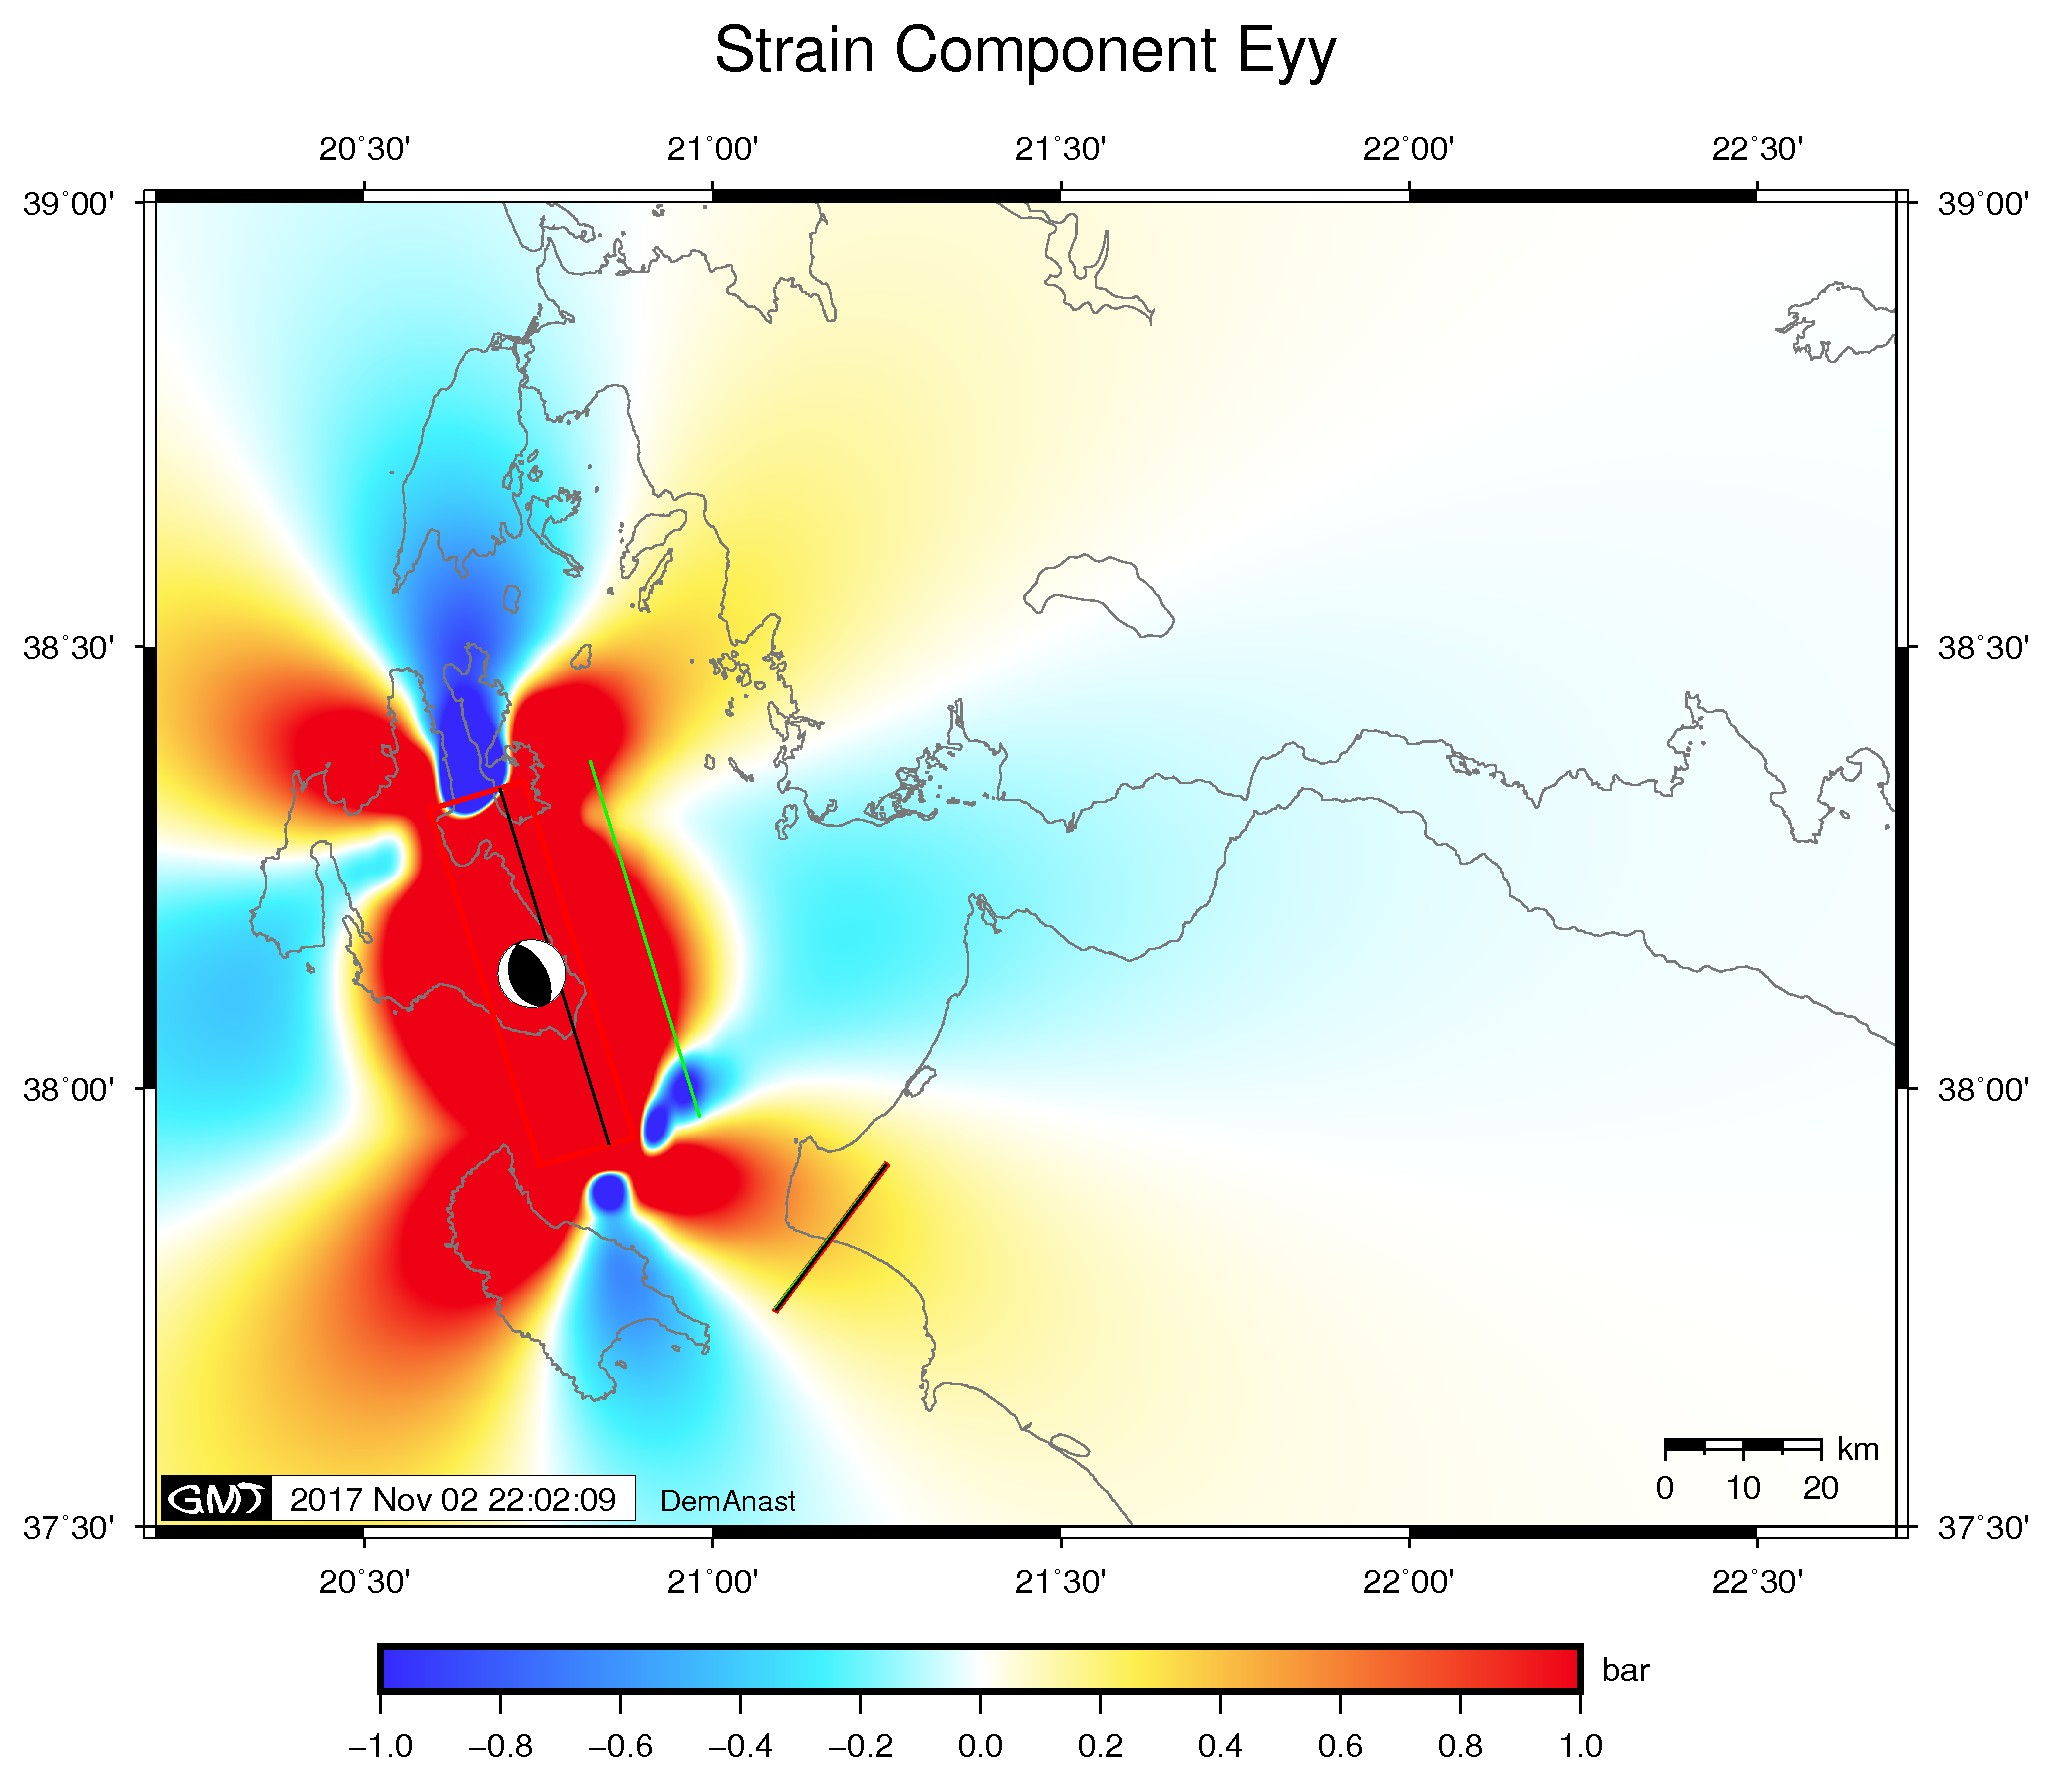
\includegraphics[width=.95\linewidth]{example504.jpg}
  \end{column}
\end{columns}

\end{frame}
\note{}

% //////////////////////////////////////////////////////////////////////////////
\begin{frame}[t,fragile]
  \frametitle{Dilatation (Exx + Eyy + Ezz) and cross section}
  \framesubtitle{Example 505}
  \label{ch5fr:ex505}
\begin{columns}[t]
  \begin{column}{.5\textwidth}
\begin{scriptsize}
\begin{verbnobox}[\vbdelim]
\$ ./coulomb2gmt.sh kef_1953 kef_1953_kef \
                   -outjpg \ 
                   --output example505 \
                   --logo_gmt \
                   --moment_tensor historic.cmt \
                   -fproj \
                   -fsurf \
                   -fdep \
                   -strdil+ot \
                   <[red]-fcross>
\end{verbnobox}
\end{scriptsize}

  \end{column}
  \begin{column}{.5\textwidth}

\centering
  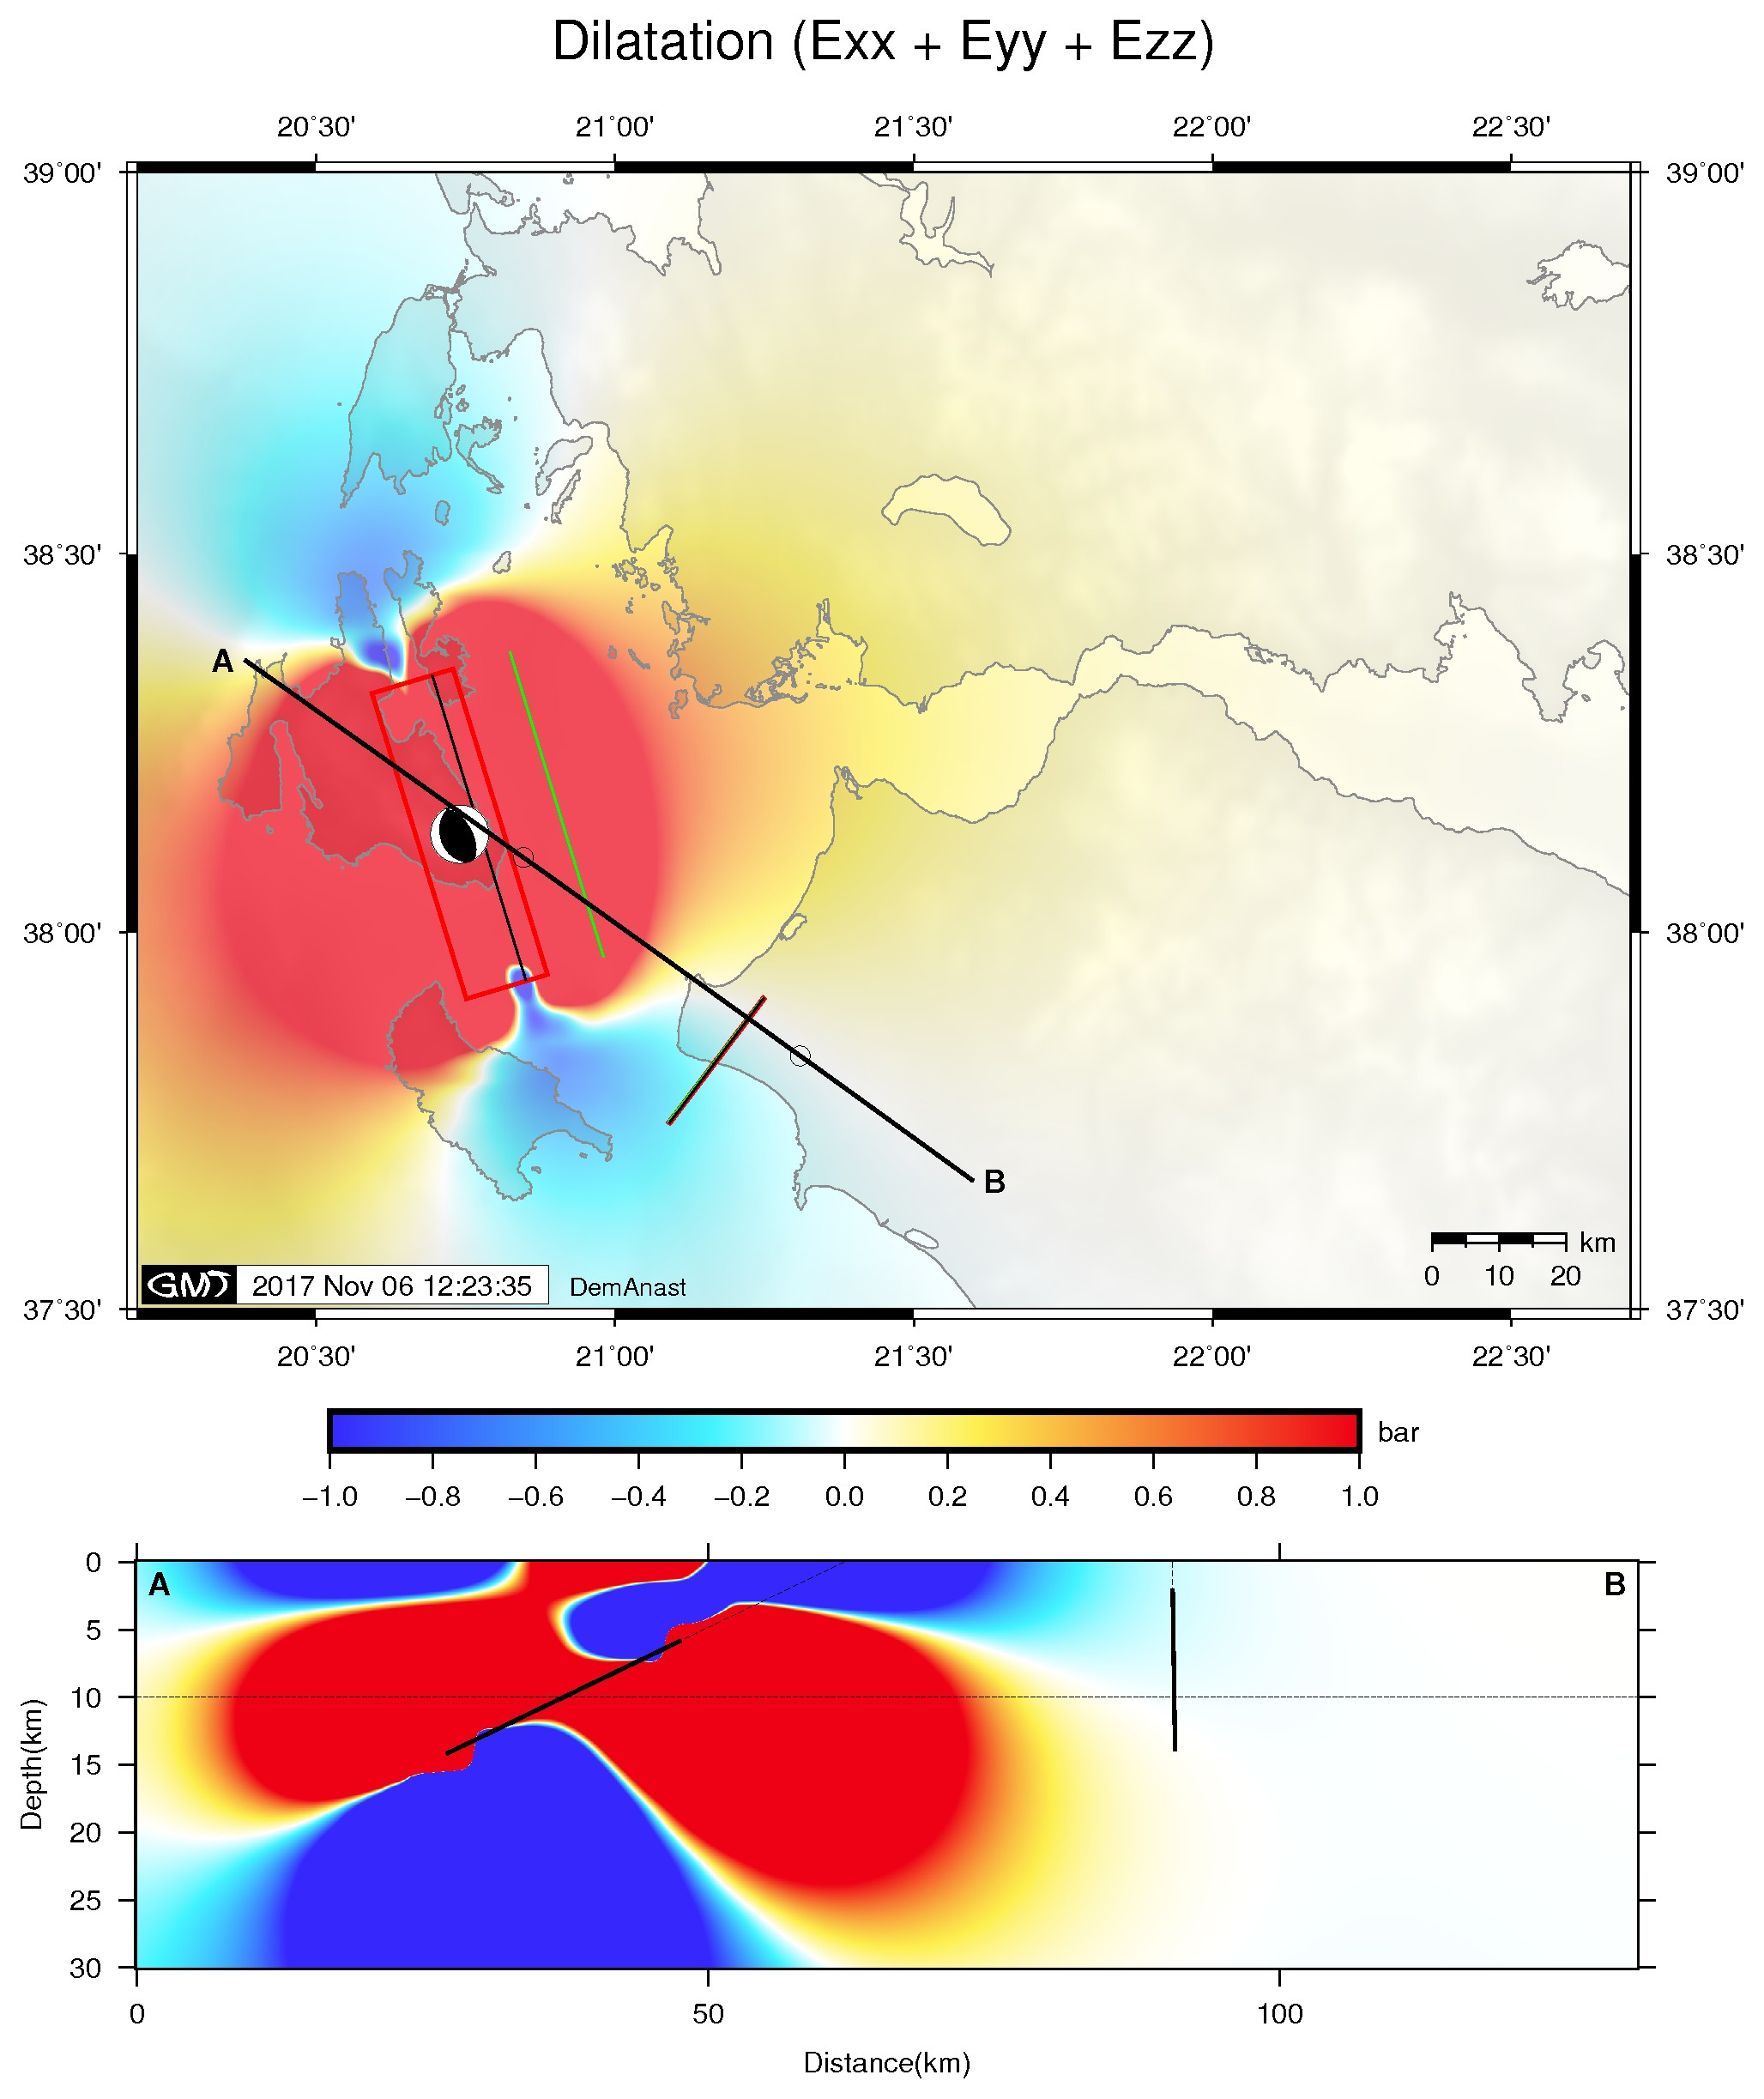
\includegraphics[width=.75\linewidth]{example505.jpg}
  \end{column}
\end{columns}

\end{frame}
\note{}





















\section[Displacements]{Displacements}

\graphicspath{{Chapter6/Figs/}}

\begin{frame}
  \frametitle{Displacements}
  \framesubtitle{}
  \label{fr6:terr_sat_ext}

\begin{itemize}
\item
  \texttt{-dgpsho}: Observed GPS horizontal displacements.
\item
  \texttt{-dgpshm}: Modeled horizontal displacements on GPS sites (Okada
  1985).
\item
  \texttt{-dgpsvo}: Observed GPS vertical desplacements.
\item
  \texttt{-dgpsvm}: Modeled vertical displacements on GPS sites (Okada
  1985).
\end{itemize}

\end{frame}
\note{}

% //////////////////////////////////////////////////////////////////////////////
\begin{frame}[t,fragile]
  \frametitle{Horizontal observe and modeledd displacements}
  \framesubtitle{Example 601}
  \label{ch5fr:ex601}
\begin{columns}[t]
  \begin{column}{.5\textwidth}
\begin{scriptsize}
\begin{verbnobox}[\vbdelim]
\$ ./coulomb2gmt.sh inp_kefa14 kefa14_ex \
                   -outjpg \ 
                   --output example601 \
                   --logo_gmt \
                   --moment_tensor historic.cmt \
                   -fproj \
                   -fsurf \
                   -fdep \
                   <[red]-dgpsho \>
                   <[red]-dgpshm >
\end{verbnobox}
\end{scriptsize}

  \end{column}
  \begin{column}{.5\textwidth}

\centering
  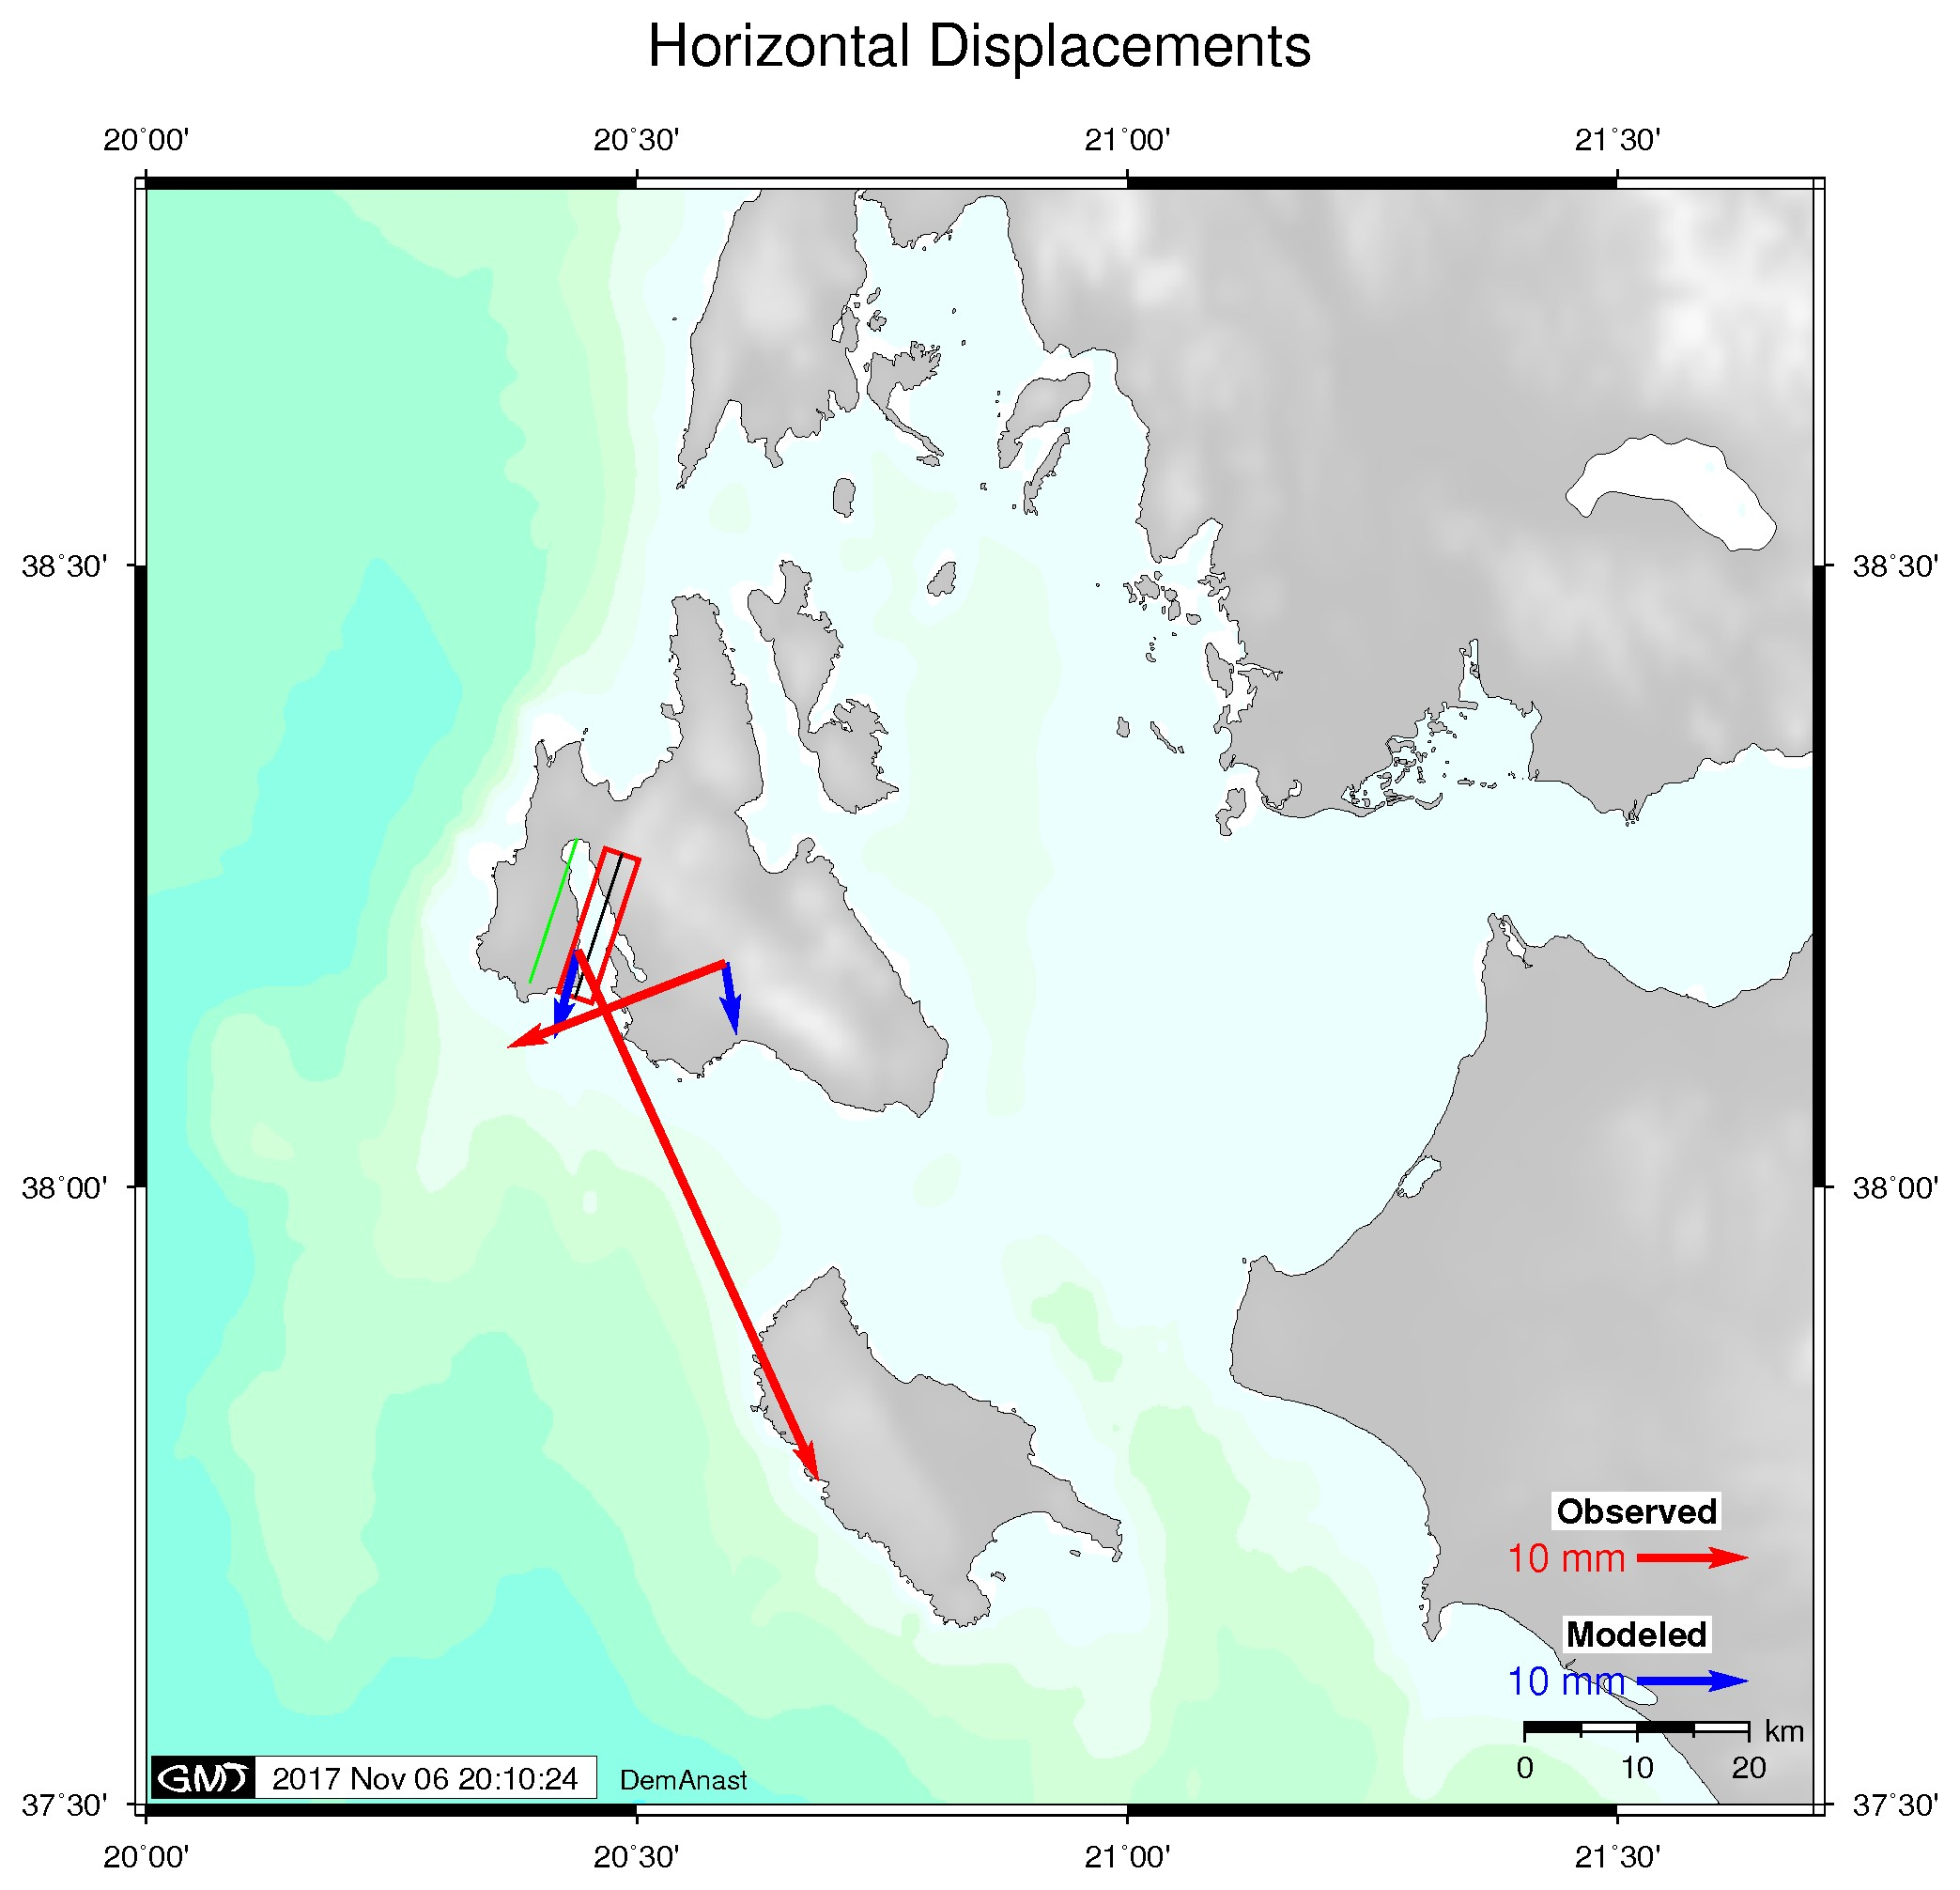
\includegraphics[width=.9\linewidth]{example601.jpg}
  \end{column}
\end{columns}

\end{frame}
\note{}

% //////////////////////////////////////////////////////////////////////////////
\begin{frame}[t,fragile]
  \frametitle{Vertical observe and modeledd displacements}
  \framesubtitle{Example 602}
  \label{ch5fr:ex602}
\begin{columns}[t]
  \begin{column}{.5\textwidth}
\begin{scriptsize}
\begin{verbnobox}[\vbdelim]
\$ ./coulomb2gmt.sh inp_kefa14 kefa14_ex \
                   -outjpg \ 
                   --output example602 \
                   --logo_gmt \
                   --moment_tensor historic.cmt \
                   -fproj \
                   -fsurf \
                   -fdep \
                   <[red]-dgpsvo \>
                   <[red]-dgpsvm >
\end{verbnobox}
\end{scriptsize}

  \end{column}
  \begin{column}{.5\textwidth}

\centering
  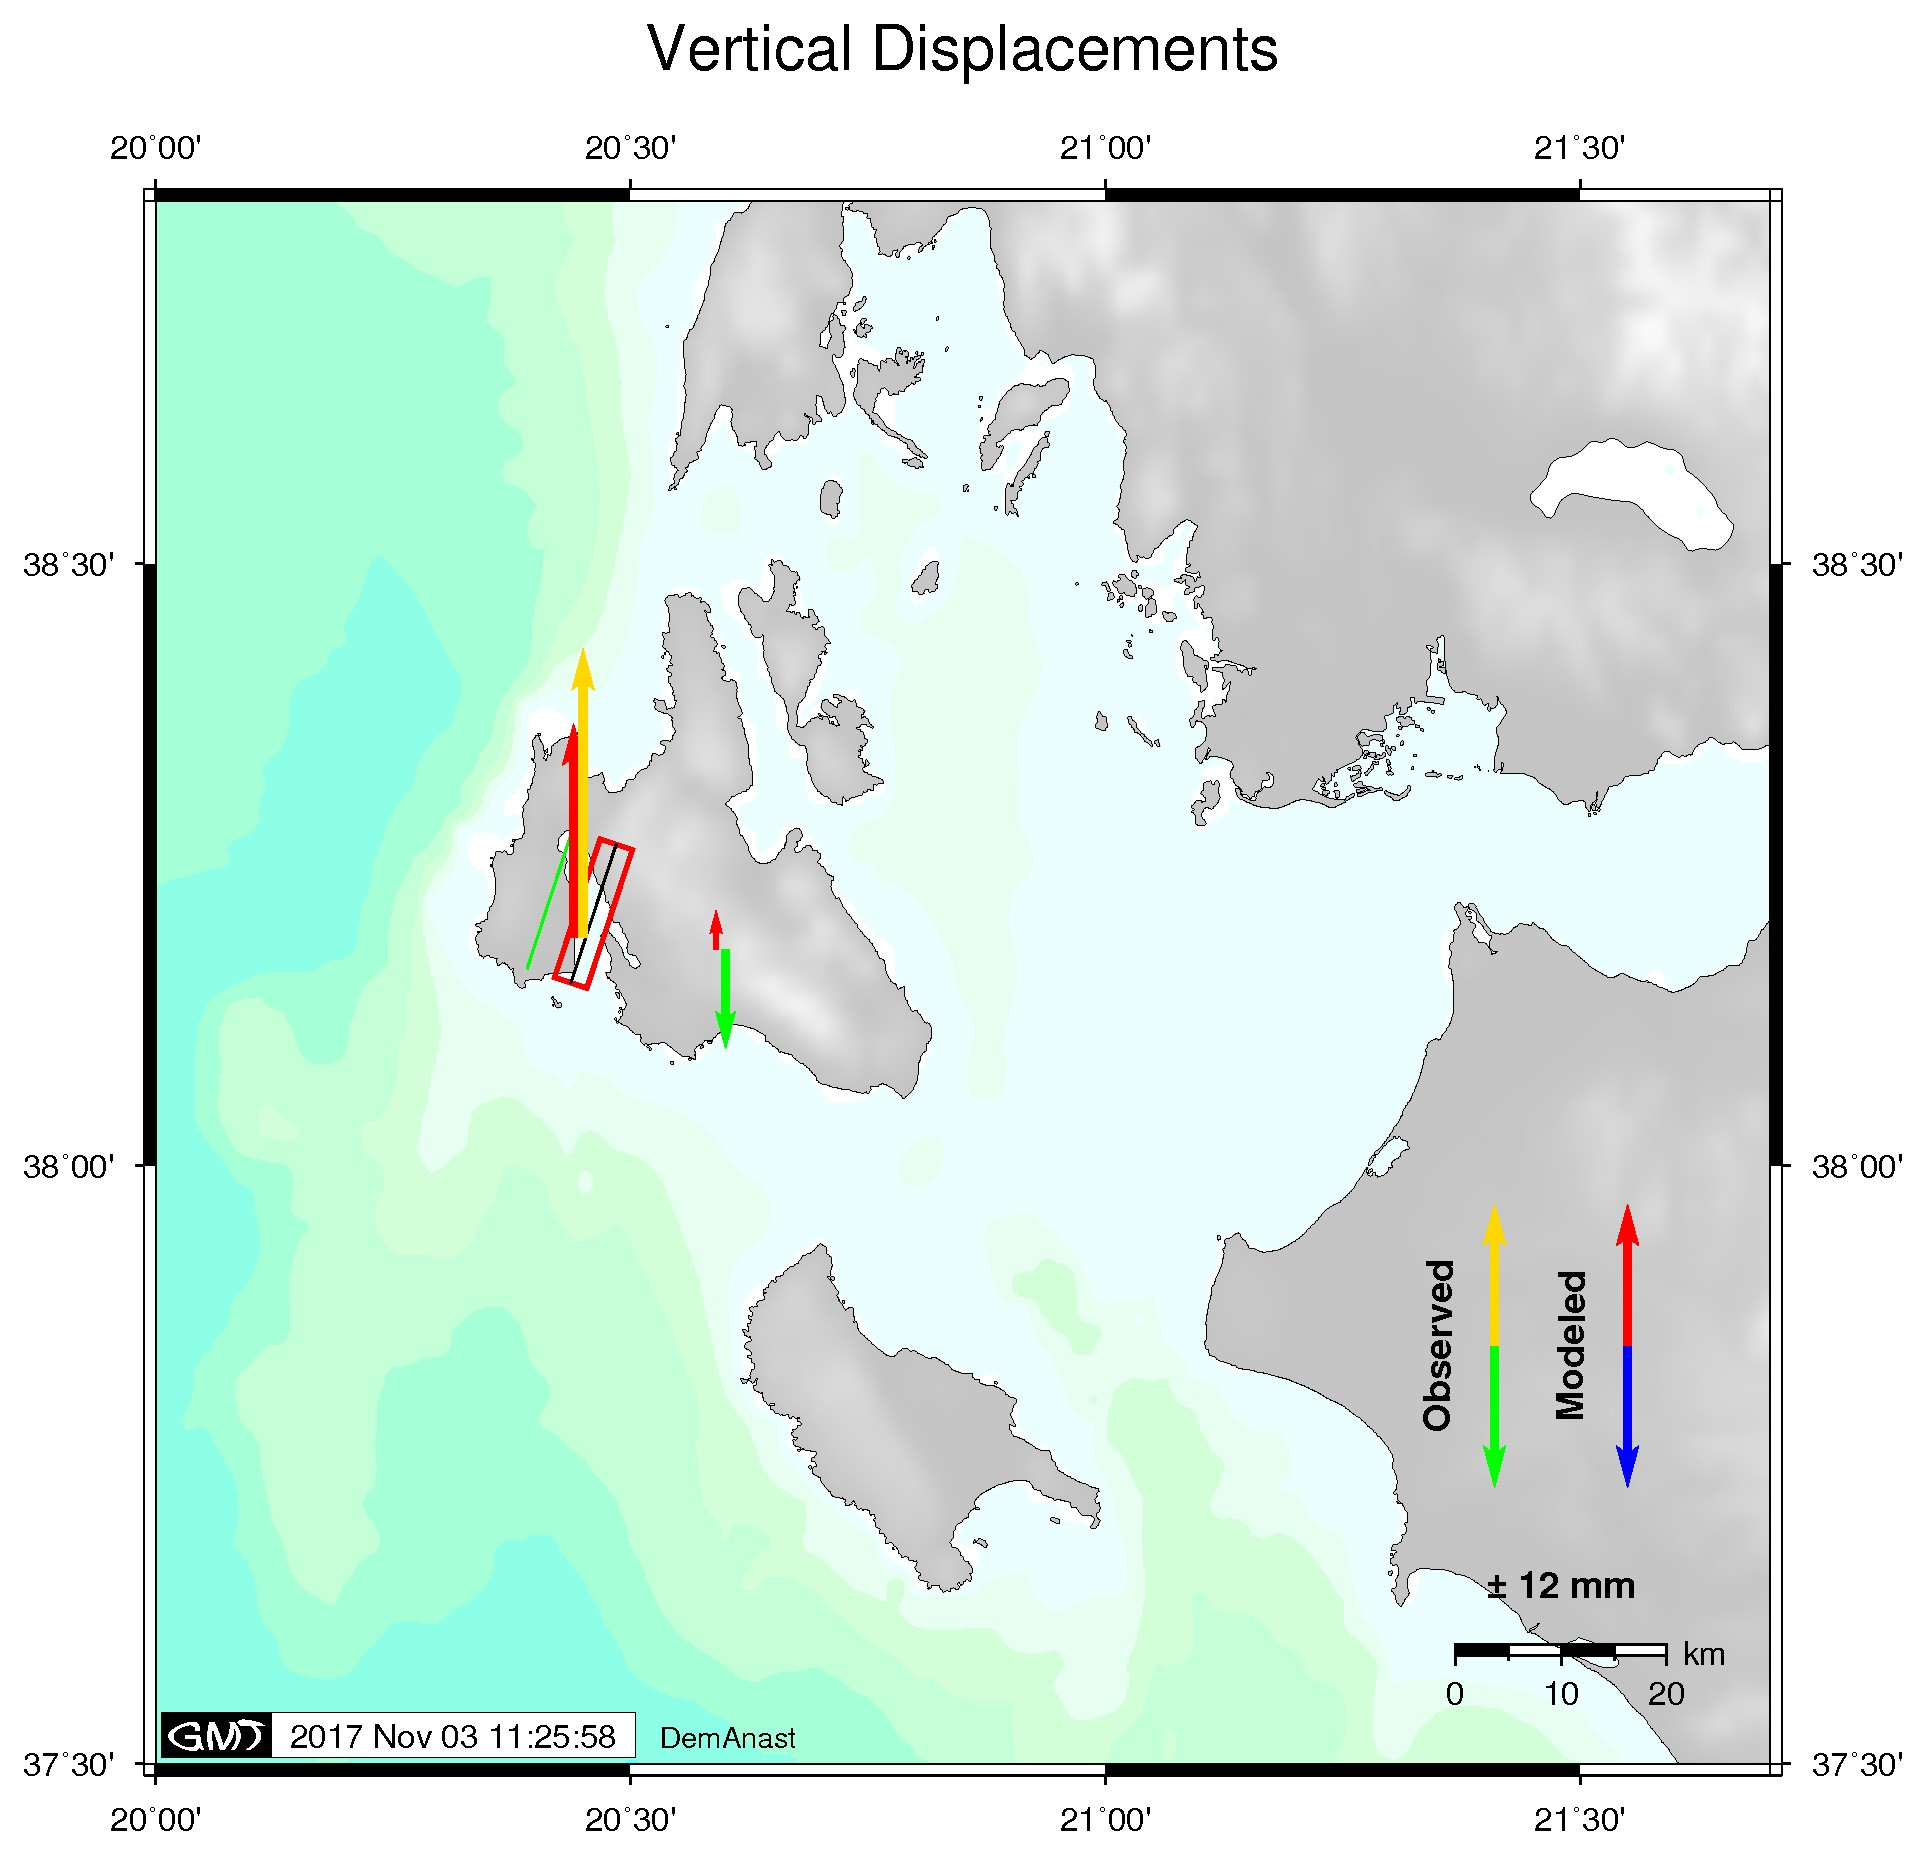
\includegraphics[width=.9\linewidth]{example602.jpg}
  \end{column}
\end{columns}

\end{frame}
\note{}

% % \section{Δημοσιεύσεις  - Λογισμικό}

\begin{frame}
  \frametitle{Δημοσιευμένες εργασίες}
  \framesubtitle{}

  
\begin{scriptsize}
    \begin{itemize}
\item[\faFile] Anastasiou D., Chouliaras G., Papanikolaou X., Marinou A., Zacharis V., Galanis J., Drakatos G., Paradissis D. (2015) \textbf{Geodetic and seismological analysis of the January 26, 2014 Cephalonia Island earthquake sequence.}  \textit{26th General Assembly of the IUGG,Prague, Czech Republic, 22/6 - 2/7.}\\
  \item[\faFile] Ganas A., Marinou A., Anastasiou D., Paradissis D., Papazissi K., Tzavaras P. and Drakatos G. (2013). \textbf{GPS-derived estimates of crustal deformation in the central and North Ionian Sea, Greece: 3-yr results from NOANET continuous network data.} \textit{Journal of Geodynamics 67, Pages 62–71A, DOI:\url{10.1016/j.jog.2012.05.010}}\\
    \item[\faFile] Papazissi K., Anastasiou D., Marinou A., Mitsakaki C., Papanikolaou X., Paradissis D. (2010) \textbf{Deformation studies in the Gulf of Patras, Western Greece.} \textit{Honorary Volume in honor of D.Arabelo, Professor of the Aristotle University of Thessaloniki.}\\
    \item[\faFile] Anastasiou D., Marinou A., Mitsakaki C., Papazissi K., Papanikolaou X., Paradissis D. (2010). \textbf{Crustal Deformation in the Patras Gulf, Greece, from GPS Data Analysis.} \textit{15th General Assembly of Wegener, Istanbul, Turkey, 14 – 17 September.}\\
  \end{itemize}
  \end{scriptsize}

\end{frame}

% % \section{Συμπεράσματα}

\begin{frame}
  \frametitle{Ρουτίνες λογισμικού}
  \framesubtitle{}
\underline{\textbf{Αποθετήριο OS code}: \href{https://github.com/demanasta}{https://github.com/demanasta \faGithub}}
\vskip.2cm
\begin{footnotesize}
Το λογισμικό έχει αναπτυχθεί στα πλαίσια της διδακτορικής διατριβής και των ερευνητικών δραστηριοτήτων του Κέντρου Δορυφόρων Διονύσου και του Εργαστηρίου Ανώτερης Γεωδαισίας και διατίθεται υπό την άδεια GPL-v3.0 ως ελεύθερο λογισμικό/λογισμικό ανοιχτού κώδικα (ΕΛ/ΛΑΚ).
\vskip.3cm
\begin{tabular}{l p{9cm}}
\textbf{1. GeoToolbox:} & Ρουτίνες σε περιβάλλον Matlab για την ανάλυση των τεκτονικών ταχυτήτων και των υπολογισμό τανυστών ανηγμένης παραμόρφωσης (\href{http://demanasta.github.io/GeoToolbox/}{http://demanasta.github.io/GeoToolbox/}) \\
\textbf{2. gpsvel:} & Σχεδιασμός χαρτών τεκτονικών ταχυτήτων και τανυστών ανηγμένης παραμόρφωσης σε περιβάλλον GMT (\href{http://demanasta.github.io/gpsvel/}{http://demanasta.github.io/gpsvel/}) \\
\textbf{3. plot\_eq:} & Σχεδιασμός χαρτών καταλόγων σεισμών στην περιοχή της Ελλάδας (\href{http://demanasta.github.io/plot\_eq/}{http://demanasta.github.io/plot\_eq/}) \\
\textbf{4. GNSS\_nets:} & Σχεδιασμός χαρτών απεικόνισης δικτύων GNSS και αποτελεσμάτων της επεξεργασίας σε περιβάλλον GMT (\href{http://demanasta.github.io/GNSS\_nets/}{http://demanasta.github.io/GNSS\_nets/}) \\
\end{tabular}
\end{footnotesize}
\end{frame}


%%-----------------------------------------------------------------------------
%% END OF PRESENTATION ...
%%-----------------------------------------------------------------------------

% ************************  Q & A frame ***************************************
% include Q&A frame at the end of presentation
\makeqahour

% ************************  Thank you frame  **********************************
% include Thank U last frame
% \makethanku % Ιncluded to class file

% ************************  Bibliography  *************************************
% % % Add 'printbib' option in Class file to Include Bibliography
\ifdefinePrintbib
  \begin{frame}[t,allowframebreaks]
    \frametitle{Βιβλιογραφία}
    \printbibliography
  \end{frame}
\fi

% ************************  Cut Frames  **************************************
% Add back up cut frames
% % \section{Κομμένα}

\graphicspath{{Chapter2/Figs/Vector/}}

% ----------------------------------------------------------------------------
% % CHAPTER 2
%-----------------------------------------------------------------------------

\begin{frame}
  \frametitle{Back frames}
  \label{frcut:backframes}

Πρόσθεσε εδώ frames σαν παράρτημα τη παρουσίασης στη περίπτωση που χρειαστούν κατά τη διάρκεια της ομιλίας.

\end{frame}
\note{}













% *********************** end of document ************************************
\end{document}
